\documentclass[12pt,oneside]{report}
\usepackage[utf8]{inputenc}
\usepackage{geometry}
\geometry{letterpaper, margin=1in}
\usepackage{graphicx}
\usepackage{setspace}
\usepackage{titlesec}
\usepackage{cite}
\usepackage{amsmath}
\usepackage{amssymb}
\usepackage{hyperref}
\usepackage{tabularx}
\usepackage{tikz}
\usetikzlibrary{positioning,shapes.geometric}
\usepackage{algorithmic}
\usepackage{pgfplots}
\pgfplotsset{compat=1.18} % This natively centers the text and prevents cumulative addition
\usepackage{booktabs}
\usepackage{float}

\newcommand{\thesisfigure}[2]{%
    \IfFileExists{#1}{\includegraphics[width=#2]{#1}}{%
        \fbox{\parbox[c][0.18\textheight][c]{#2}{\centering Figure asset ``#1'' was not available at compilation time.}}%
    }%
}

\doublespacing

\begin{document}

% --- Title Page ---
\begin{titlepage}
    \centering
    \vspace*{1.5cm}
    
    {\Large \bfseries An Agentic Research System and Interactive Flywheel for Long-Tail Healthcare Resource Discovery\par}
    \vspace{1.5cm}
    
    A Thesis Submitted to the\par
    School of Graduate Studies\par
    In Partial Fulfillment of the Requirements\par
    For the Degree of Master of Science in Computer Science\par
    Algoma University\par
    Brampton, Ontario, Canada\par
    
    \vspace{2cm}
    By\par
    \vspace{1cm}
    {\large \bfseries Kevin Igweh\par}
    
    \vspace{2cm}
    \vspace{1.5cm}
    {\small \copyright\ Copyright Kevin Igweh, 2026. All rights reserved.\par}
\end{titlepage}

% --- Permission to Use / Disclaimer ---
\newpage
\thispagestyle{empty}
\chapter*{Permission to Use}
\addcontentsline{toc}{chapter}{Permission to Use}
In presenting this thesis in partial fulfillment of the requirements for a Postgraduate degree from Algoma University, I agree that the Libraries of this University may make it freely available for inspection. I further agree that permission for copying of this thesis in any manner, in whole or in part, for scholarly purposes may be granted by the professor or professors who supervised my thesis work or, in their absence, by the Head of the Department or the Dean of the Faculty in which my thesis work was done. It is understood that any copying or publication or use of this thesis or parts thereof for financial gain shall not be allowed without my written permission. It is also understood that due recognition shall be given to me and to Algoma University in any scholarly use which may be made of any material in my thesis.

\newpage
\chapter*{Acknowledgements}
\addcontentsline{toc}{chapter}{Acknowledgements}

I would like to express my deepest gratitude to my supervisors, \textbf{Professor Wenjun Lin} and \textbf{Professor Ajmery Sultana}, for their invaluable guidance, constant encouragement, and insightful feedback throughout this research journey. Their wisdom, technical expertise, and unwavering support were instrumental in shaping this thesis and pushing me to achieve academic excellence.

I am immensely grateful to my dear friends and academic colleagues, \textbf{Jikesh Thapa} and \textbf{Serban Voinea Gabrean}, for their camaraderie, engaging intellectual discussions, and continuous support during long research sessions. Their presence made this journey far more enriching and memorable.

My heartfelt thanks go to my family, whose love, prayers, and sacrifices have been the bedrock of my success. To my father and mother, \textbf{John and Florence Igweh}, thank you for your unconditional love, endless belief in my abilities, and the foundation you provided me. To my wonderful sisters—\textbf{Linda, Mildred, Jane, and Vanessa Igweh}—thank you for always keeping me grounded, bringing joy into my life, and cheering me on every step of the way. 

I also extend my sincere appreciation to my uncle and aunt, \textbf{Nathan and Ayo Ogor}, for their continuous encouragement, guidance, and steady support throughout my academic pursuits.

Above all, I thank Almighty God for the strength, wisdom, and perseverance to complete this milestone.

% --- Abstract ---
% --- Abstract ---
\chapter*{Abstract}
\addcontentsline{toc}{chapter}{Abstract}
Effective care coordination requires healthcare professionals to connect patients with community-based services that complement clinical treatment—local programs spanning rehabilitation, social support, and specialized care. However, these vital resources are highly fragmented across the web, leaving discharge planners and social workers without a comprehensive inventory of operational services in their region. Existing automated approaches can fail this task because Large Language Model (LLM) query generation may collapse toward high-frequency phrasings. This systematic failure—a phenomenon we term \textit{generative convergence}—can force search agents into an "SEO trap," causing them to miss small, hyper-local, weakly indexed community services that matter most for integrated care. This thesis addresses this data-discovery problem through the Agentic Research System (ARS).

The ARS formalizes community healthcare mapping as a long-tail retrieval problem. Here, a long-tail domain is one in which a small number of highly visible organizations account for much of the searchable content while many valid services appear infrequently across local pages, PDFs, and directories. The ARS uses a four-axis Query Expansion Matrix (QEM)—entity, scope, attribute, and source—to decouple query diversity from LLM sampling through deterministic template permutations. Retrieved web data flows through extraction, entity resolution, and a three-stage evidence pipeline combining registry matching, domain-targeted search, and API signals. Manual review establishes the extended ground truth for entities absent from the baseline registries. Benchmarked against three curated datasets (addiction counseling, hospitals, and pharmacy services), the ARS achieved 78.3\% average baseline recall and surfaced additional manually verified resources absent from the reference inventories.

To address the subsequent maintenance problem, Project 2 introduces Pathways, an interactive service-search and directory-maintenance platform. Pathways uses an event-sourced data model and a Find--Verify--Ask--Close flywheel to capture human validation and support longitudinal directory maintenance. Four focused evaluations characterize the combined system. The structured 200-query extraction benchmark evaluated five conditions: basic rules achieved micro-F1 of 0.892, aliases 0.932, semantic-only extraction 0.966, Gemini-only extraction 0.989, and semantic plus Gemini 1.000. These results are development-fixture evidence rather than held-out estimates because the ontology and query families were used during implementation. On an independently adjudicated ranking set, BM25 achieved higher nDCG@5 than the current Pathways ranker (0.916 versus 0.804). A simulated participation sweep showed that day-90 freshness increased from 0.00 with no verification participation to 1.00 under full participation. Finally, the Pathways Data Restoration benchmark classified 142 of 500 requested fields as exact, 284 as supported non-exact values, 63 as weakly supported, and 11 as unresolved after manual review. These results support Pathways as an auditable maintenance prototype, while identifying language coverage, ontology calibration, ranking calibration, simulation realism, and source-level validation as limitations.

% --- Table of Contents ---
\tableofcontents
\newpage

% 2. List of Figures
\phantomsection 
\addcontentsline{toc}{chapter}{\listfigurename} 
\listoffigures
\clearpage

% 3. List of Tables
\phantomsection 
\addcontentsline{toc}{chapter}{\listtablename} 
\listoftables
\clearpage

% --- CHAPTER 1 ---
\chapter{Introduction}

\section{Background}

\subsection{The Landscape of Care Coordination and Community Resources}
Modern healthcare delivery increasingly treats patient outcomes as the result of both clinical treatment and the conditions in which patients live. Social determinants of health (SDoH), including housing, transportation, social support, income, and access to community services, shape whether a patient can follow a treatment plan after leaving a hospital or clinic. Care coordination therefore extends beyond the clinical encounter. It requires professionals to identify appropriate services, determine whether those services are operating, and connect a patient with an organization that can respond to the patient's practical circumstances \cite{44,45}.

This task is particularly important during discharge and referral workflows. A discharge planner or social worker may need to locate addiction counseling, peer-support groups, rehabilitation programs, specialized care, or pharmacy services within a particular geographic area. The relevant resource may be a large institution, but it may also be a small organization with limited online visibility, a program embedded in a larger community organization, or a service described only in a local directory or document. The quality of a referral is therefore determined not only by whether an organization exists, but also by whether the service type, location, contact information, eligibility requirements, and operating status match the patient's needs.

Community healthcare resource discovery is consequently a data-integration problem as well as a clinical coordination problem. Information is distributed across municipal registries, institutional websites, commercial listings, nonprofit pages, social-care portals, and documents published in different formats. These sources use inconsistent names and descriptions, provide different levels of detail, and often describe the same organization from different perspectives. A useful discovery system must combine these heterogeneous signals into records that can be searched and compared without removing the provenance needed to assess their reliability.

\subsection{The Fragility of Manual Directories}
Despite their importance, community resources are not represented by one stable, complete, and consistently maintained information system. A service may change its telephone number, intake process, hours, eligibility criteria, or website without those changes appearing simultaneously in every directory. Organizations may also open, merge, relocate, suspend a program, or stop publishing information while remaining present in older records. The resulting directory is fragile because its usefulness depends on several mutable fields remaining accurate at the same time.

Manual curation is valuable for establishing trusted reference information, but it does not scale easily to the full discovery problem. Staff must find candidate organizations, reconcile duplicates, inspect sources, update fields, and repeat the process as conditions change. This creates two related weaknesses. First, a manually maintained directory tends to prioritize sources that are already known to administrators, which can preserve visibility and geographic biases. Second, updates are expensive and sporadic, so a record can become stale between review cycles. The problem is not simply that a directory contains too few rows; it may contain the wrong level of detail or fail to communicate which fields were recently supported by evidence.

These limitations also affect clinical workload. When a directory cannot answer a referral question, the professional must conduct additional web searches, call organizations, or enter information manually into another system. The result is repeated administrative work and a loss of time during transitions of care. Community-resource referral research similarly identifies organizational and workflow barriers to implementing resource-referral technologies \cite{20}. An automated system must therefore reduce discovery effort without presenting unverified outputs as authoritative clinical recommendations.

\subsection{Automated Extraction and Generative Convergence}
To address the scale of manual discovery, recent systems use automated web navigation, language-model extraction, retrieval augmentation, and multi-agent tool use \cite{10,13,15,19,21}. These approaches are attractive because they can interpret varied language, follow a research objective, and transform unstructured pages into structured records. In principle, an LLM can recognize that different phrases refer to related services even when a page does not follow a fixed template.

The retrieval stage creates a separate problem from extraction quality. An agent must decide what to search before it can extract anything. If the model generates each next query from its own probability distribution, it is likely to reuse familiar terms and prominent organizations. Search-engine ranking can reinforce this behavior: highly linked and search-optimized pages appear early, are summarized by the agent, and then influence subsequent queries. We call this interaction the ``SEO Trap.'' It is a practical retrieval bias in which visibility is mistaken for completeness.

For example, an agent asked to find addiction-support services across a province may repeatedly issue broad queries and return a large metropolitan institution. It may correctly describe that institution while never searching for small peer-support programs, local outreach services, or organizations whose information appears only in a regional document. The agent has not necessarily made an extraction error; it has failed to construct a sufficiently diverse retrieval space. This distinction motivates the thesis definition of \textit{Generative Convergence}: the tendency of an LLM-led search process to concentrate successive queries and results around high-frequency terminology and already-visible entities, reducing exploration of the long tail.

In this thesis, a long-tail domain is one where a relatively small searchable ``head'' contains highly visible organizations, while many valid resources are distributed across lower-population areas and heterogeneous, weakly indexed sources. Long-tail fragmentation describes the second property: the resources are not merely less popular, but scattered across many pages, documents, naming conventions, and geographic contexts. An automated system that produces many records from the head can therefore appear productive while still leaving important parts of the service network undiscovered.

\subsection{The Socio-Technical Challenge of Data Maintenance}
Reducing retrieval bias does not by itself produce a permanently reliable directory. Community services change over time, and the information extracted during one run can become outdated. This creates a second problem: how can an initial inventory be maintained without requiring professionals to repeatedly rebuild it manually? A directory is useful only when its users can understand the evidence behind a record, identify stale fields, and correct errors with an acceptable amount of effort.

This is a socio-technical challenge because technical accuracy and user behavior are connected. A system that returns many candidates but gives no indication of their evidence may reduce trust. A system that requires lengthy forms or separate administrative workflows may be ignored. Conversely, a workflow that places small verification actions close to the user's normal search activity can make maintenance more feasible. Human-in-the-loop research emphasizes that human participation is particularly important when automated decisions affect complex or high-stakes domains \cite{47,48,51}.

Pathways addresses this maintenance layer by providing an interactive interface around the ARS output. Its event-sourced model records changes rather than silently overwriting them, while the Find--Verify--Ask--Close flywheel connects searches, field verification, issue reports, and ARS-assisted updates. The design does not assume that automation can replace human judgment. Instead, it treats ARS as a discovery and enrichment component and treats human review as necessary for decisions that affect the trusted directory state.

\section{Research Gaps and Thesis Response}
The background establishes a problem that cannot be addressed by extraction accuracy alone. Existing LLM and multi-agent web systems demonstrate strong reasoning and tool-use capabilities, but their retrieval procedures commonly leave query selection to the model. This makes it difficult to determine whether a system failed because a resource was absent, because the search engine ranked it poorly, or because the agent never issued a query capable of finding it. Existing web-agent benchmarks also emphasize task completion in structured and navigable environments, which does not directly measure coverage of fragmented community healthcare resources \cite{10,11,12,15}. The first gap addressed by this thesis is therefore the under-specification of retrieval diversity in long-tail healthcare discovery.

A related gap arises from treating discovery and extraction as a single problem. An agent may extract accurately from a page it has already found while still producing poor overall coverage. Conversely, a broad crawler may collect many pages while producing inconsistent or duplicated records. The literature provides useful extraction and grounding techniques \cite{30,36,37,40,41}, but the relationship between deterministic query-space construction, heterogeneous web retrieval, schema extraction, and entity resolution requires more explicit evaluation in community healthcare settings. Project 1 responds by separating these stages in the Agentic Research System (ARS): the Query Expansion Matrix (QEM) constructs the query space, web collection retrieves candidate material, language-model extraction imposes a schema, and the entity-resolution pipeline consolidates overlapping records.

The third gap concerns how long-tail coverage is evidenced. Raw output volume is not sufficient evidence of broad discovery. A system that returns more records may simply be less selective, while a system with high precision may still miss low-visibility services. Evaluation must therefore combine baseline matching with independent verification of novel candidates, geographic distribution, error categories, and workflow-level measurements. Without this extended evaluation, valid discoveries absent from a registry can be incorrectly counted as failures, while unverified or out-of-scope records can be mistaken for success. The ARS evaluation responds through baseline recall, precision and error analysis, geographic stratification, workflow throughput measurements, and an extended ground-truth protocol for candidates absent from the reference inventories.

The final gap is the weak connection between initial discovery and longitudinal maintenance. Automated discovery addresses the cold-start problem, but directories also require correction as organizations and services change. Human-in-the-loop systems and event-sourced designs offer principles for preserving provenance and incorporating feedback \cite{47,48,55,56,57}; however, these principles must be connected to a practical healthcare-resource workflow in which automated discoveries can be reviewed, enriched, and maintained without being presented as clinically authoritative. Project 2 responds through Pathways, which provides an event-sourced ledger, a derived projection, and a human-facing Find--Verify--Ask--Close workflow. Its targeted missing-data restoration study evaluates how effectively the connected workflow can recover incomplete organizational information.

The thesis is consequently structured around two complementary responses to the same information problem. ARS addresses breadth, retrieval diversity, extraction, entity resolution, and evidence collection, while Pathways addresses provenance, human verification, ranking, and continued maintenance. Together, the projects investigate how a broad inventory of decentralized healthcare resources can be constructed without allowing generative search bias to determine what is discoverable and how that inventory can remain useful as information changes. Neither system is presented as a guarantee of complete provincial coverage or as a replacement for authoritative registries and clinical judgment; rather, the thesis evaluates whether structural query diversity, evidence-based verification, and human-mediated maintenance provide a more appropriate foundation for this class of healthcare information task.

\section{Research Objectives}
The primary objective of this thesis is to address the discovery and longitudinal maintenance of decentralized community healthcare resources on the open web through two connected systems: ARS and Pathways.

Specifically, this research pursues the following core objectives:
\begin{enumerate}
    \item To formalize the failure of generative search architectures in mapping long-tail domains by defining and empirically demonstrating the phenomenon of \textit{Generative Convergence}.
    \item To engineer an autonomous extraction pipeline—the Agentic Research System (ARS)—that uses deterministic query enumeration, semantic extraction, entity resolution, and evidence-based verification to discover hyper-local healthcare data from the open web.
    \item To quantify ARS coverage, verified novel discoveries, workflow throughput, geographic distribution, and error categories across three healthcare domains.
    \item To compare ARS with commercial generative systems and tool-augmented or multi-agent alternatives, while identifying the limits of the available comparisons.
    \item To design and evaluate Pathways, an event-sourced, human-in-the-loop platform for maintaining and ranking discovered healthcare resources over time.
\end{enumerate}

\section{Organization of the Thesis}
The remainder of this thesis is structured as follows:
\begin{itemize}
    \item \textbf{Chapter 2 (Literature Review):} Reviews autonomous web navigation, long-tail retrieval, information extraction, entity resolution, and tool-augmented alternatives relevant to ARS.
    \item \textbf{Chapter 3 (The Agentic Research System):} Details the ARS architecture, Query Expansion Matrix, entity-resolution pipeline, verification protocol, and empirical evaluation.
    \item \textbf{Chapter 4 (Pathways):} Introduces the interactive directory-maintenance platform, its event-sourced architecture, maintenance flywheel, and evaluation design.
    \item \textbf{Chapter 5 (Conclusion and Future Work):} Summarizes the findings, limitations, privacy considerations, and directions for improving ARS and Pathways.
\end{itemize}

% --- CHAPTER 2 ---
\chapter{Literature Review}

\section{Introduction}
This chapter reviews the technical foundations of the Agentic Research System (ARS) as a discovery pipeline. First, we examine autonomous web navigation and identify \textit{Generative Convergence}, the failure mode that the ARS is designed to test and mitigate. Second, we examine extraction from unstructured web environments and entity resolution, which support the ARS's semantic filtering and deduplication stages. Finally, we review tool-augmented and multi-agent alternatives used as architectural and empirical comparison points.

\section{Autonomous Web Navigation and Generative Convergence}
The automation of information gathering has fundamentally shifted from static, rule-based web scraping \cite{1, 2} to dynamic, autonomous web navigation powered by Large Language Models (LLMs) \cite{3, 4, 5}. While traditional scraping architectures require rigid, human-engineered DOM parsers that break upon minor website updates, modern systems leverage the zero-shot reasoning capabilities of foundation models \cite{6, 7} to dynamically formulate search queries and navigate complex environments. 

\subsection{Single-Loop and Environment-Grounded Agents}
Early iterations of LLM-driven navigation, such as WebGPT \cite{10}, introduced the paradigm of coupling a language model directly to a text-based web browser. To standardize the evaluation of these autonomous behaviors, frameworks like WebArena \cite{11} and AgentSims \cite{12} were developed to situate LLMs in highly realistic, reproducible web environments. While these benchmarks effectively measure task completion across structured domains like e-commerce and forums, their evaluation metrics implicitly presuppose navigable, well-organized site architectures. The idiosyncratic, unstructured, and deeply buried directories characteristic of long-tail Social Determinants of Health (SDoH) resources are entirely absent from these environments, leaving a critical gap in agentic evaluation.

\subsection{Tool-Augmented and Reasoning Frameworks}
The integration of explicit tool-use capabilities represented a significant leap forward in autonomous navigation. Frameworks such as Toolformer \cite{13}, Gorilla \cite{14}, and ToolLLM \cite{8} demonstrated that LLMs could invoke external APIs and search engines autonomously. Building upon tool integration, the ReAct (Reasoning and Acting) framework \cite{15}, alongside Chain-of-Thought prompting \cite{16} and Self-Consistency \cite{17}, became the state-of-the-practice for dynamic web agents. 

Despite this sophisticated iterative reasoning, ReAct-based agents share a critical vulnerability: the LLM itself is solely responsible for deciding what to search at each step. Because the model formulates queries by sampling from its internal probability distribution, it naturally gravitates toward high-frequency, statistically probable phrasings. In the context of this thesis, this phenomenon is formalized as \textit{Generative Convergence}—a systemic flaw where agents systematically ignore the highly specific, idiosyncratic queries required to surface tail-end resources.

\subsection{Multi-Agent Systems and the ''SEO Trap''}
Recent advancements bypass traditional HTML parsing by utilizing Large Multimodal Models (LMMs) \cite{18} and multi-agent topologies (e.g., AutoGen \cite{19}, BabyAGI \cite{20}) to collaboratively execute complex web research \cite{9}. This commercialization has culminated in "deep research" systems integrated into proprietary models like OpenAI's ChatGPT \cite{21}, Google's Gemini Advanced \cite{22}, and Anthropic's Claude \cite{23}. 

However, driven by their training distributions and augmented retrieval mechanics \cite{25}, these models may bias their search parameters toward well-indexed corporate terminology. This is the ''SEO trap'' \cite{24}: a search process returns prominent pages repeatedly because search-engine ranking and model query selection reinforce visibility. For example, an agent asked to find addiction-support services across a province may repeatedly return a large metropolitan institution while failing to issue queries for small peer-support programs in rural municipalities. During iterative search loops, the agent may then terminate after collecting prominent results, treating the topic as exhausted.

\textbf{Connection to the Proposed System:} Collectively, the existing literature reveals a shared, unexamined architectural assumption: the belief that the LLM should autonomously decide what to query. The Agentic Research System (ARS) presented in Project 1 challenges this assumption. By utilizing a deterministic Query Expansion Matrix (QEM) that forces structural variance across entity, scope, attribute, and source axes, the ARS decouples query diversity from the LLM's generative sampling and provides a reproducible strategy for broader long-tail discovery.

Table~\ref{tab:literature_synthesis} summarizes the systems reviewed in this chapter and positions the thesis contribution relative to them. The comparison distinguishes the problem each system was designed to solve from the long-tail healthcare discovery problem addressed here. In particular, a system may demonstrate strong navigation, tool use, or extraction performance without providing a mechanism for systematic query-space coverage or independent validation of newly discovered healthcare resources.

\begin{table}[htbp]
\caption{Synthesis of Reviewed Systems and the ARS Research Gap}
\label{tab:literature_synthesis}
\centering
\scriptsize
\renewcommand{\arraystretch}{1.25}
\begin{tabularx}{\textwidth}{@{}p{2.2cm} X X X X@{}}
\toprule
\textbf{System or approach} & \textbf{Primary capability} & \textbf{Typical setting} & \textbf{Limitation for long-tail healthcare discovery} & \textbf{ARS response} \\
\midrule
WebGPT \cite{10} & Browser-assisted question answering with search and reading. & Open-web question answering. & Follows a task-oriented search loop but does not structurally enumerate a sparse query space. & Separates query-space construction from language-model reading through QEM. \\
WebArena and AgentSims \cite{11,12} & Reproducible environments for evaluating web-agent behavior. & Structured websites and benchmark tasks. & Task completion in navigable environments does not directly measure fragmented community-resource coverage. & Evaluates entity coverage, geographic distribution, and verification outcomes on heterogeneous sources. \\
Toolformer, Gorilla, and ToolLLM \cite{13,14,8} & Language-model tool invocation and API use. & API- and tool-augmented language-model workflows. & Tool access does not determine which geographic, service, or source combinations should be searched. & Uses the LLM for slot filling while QEM deterministically defines the combinations. \\
ReAct \cite{15} & Iterative reasoning and action selection. & Multi-step browsing and tool use. & Successive query selection remains dependent on model generation and may converge on prominent results. & Makes query diversity an architectural constraint rather than a sampling outcome. \\
WebVoyager \cite{18} & Multimodal browser interaction and visual web navigation. & Complex interactive web pages. & Improved navigation does not by itself solve coverage, source fragmentation, or entity deduplication. & Adds structured extraction, five-layer entity resolution, and evidence-based verification. \\
AutoGen and BabyAGI \cite{19,20} & Multi-agent task decomposition and collaborative web research. & General-purpose agent coordination. & Additional agents may increase search depth without guaranteeing geographic or query diversity. & Measures the discovered inventory and uses deterministic QEM coverage across four axes. \\
Commercial deep-research systems \cite{21,22,23} & Extended browsing, retrieval, and narrative synthesis. & General research assistance. & Optimized for answer synthesis; query selection and coverage are not auditable or guaranteed. & Optimizes for structured database population, provenance, and measurable baseline coverage. \\
ARS (this thesis) & Query enumeration, web extraction, entity resolution, and verification. & Decentralized healthcare resources on the open web. & Current limitations include shallow crawling, API dependence, and the need for manual validation of novel candidates. & Addresses the identified gap while reporting these limitations explicitly. \\
\bottomrule
\end{tabularx}
\end{table}

\section{Information Extraction from Unstructured Data}
Successfully reducing Generative Convergence at retrieval does not eliminate extraction difficulty. Once an agent reaches a target page, it must overcome structural noise to parse operational data. Traditional extraction methods, such as Regular Expressions (Regex) and Named Entity Recognition (NER) \cite{26, 27}, can be brittle when applied to heterogeneous HTML structures common in community healthcare.

\subsection{LLMs as Zero-Shot Semantic Extractors}
The advent of LLMs revolutionized information extraction by shifting the paradigm from syntactic parsing to semantic understanding \cite{28, 29}. Recent literature demonstrates that LLMs frequently outperform traditional supervised models in medical contexts without requiring extensive parameter tuning \cite{30, 31, 32}. Polak and Morgan \cite{33} and Zhao et al. \cite{35} established that careful prompt design—specifically, instructing the model to output strict JSON schemas—is sufficient to impose structural compliance across highly heterogeneous source material \cite{34}.

\subsection{Grounding and Factuality in Extraction}
A persistent challenge in LLM-based extraction is the model's propensity for generative hallucination \cite{40}. To combat this, modern architectures strictly tether generation to retrieved evidence. Retrieval-Augmented Generation (RAG) \cite{36} and few-shot architectures (such as Atlas \cite{37} and REALM \cite{38}) demonstrate that forcing the model to explicitly cite retrieved passages measurably improves factual fidelity \cite{39}. Furthermore, self-verification protocols \cite{41, 42, 43} have been developed to ensure that extracted clinical entities are strictly traceable to the source text rather than the model's parametric memory.

\textbf{Connection to the Proposed System:} The ARS converts raw HTML to standardized Markdown and uses strict JSON alignment prompting before applying external evidence checks. Automated signals support triage, while manual review establishes the extended ground truth for candidates absent from baseline registries.

% --- CHAPTER 3 ---
\chapter{An Agentic Research System for Long-Tail Healthcare Resource Discovery}
\section{Introduction}

Modern healthcare delivery relies heavily on community-based services that operate outside the traditional walls of the clinic. Effective care coordination and hospital discharge planning fundamentally depend on access to accurate, up-to-date directories of these local resources, which include specialized rehabilitation, peer support, and marginalized population care. However, the sheer fragmentation of the community health ecosystem presents a massive operational bottleneck. As recent literature on health and human services integration has established, the manual curation and maintenance of these hyper-local directories is administratively prohibitive, resulting in tools that rapidly decay in clinical utility and fail to address core Social Determinants of Health (SDoH) \cite{44, 45}.

To overcome the limitations of manual curation, researchers and health informaticians have increasingly turned to Large Language Models (LLMs) to autonomously navigate the web and aggregate unstructured data \cite{28, 30}. While LLMs excel at semantic synthesis and have demonstrated utility in automated dataset creation, they exhibit a systemic failure mode when tasked with finding hyper-local community services. As established in Chapter 2, because their underlying probability distributions inherently favor high-frequency training data, LLM query generation naturally collapses toward well-indexed, corporate healthcare networks. They systematically miss the decentralized, weakly indexed community nodes that are most vital for integrated care. 

This phenomenon, formalized in this thesis as \textit{Generative Convergence}, forces conversational agents into an "SEO Trap" \cite{24, 25}. By allowing the LLM to autonomously decide \textit{what} to search for, current frameworks may concentrate on dominant medical organizations and under-sample the long-tail ecosystem required by healthcare navigators. In this thesis, long-tail fragmentation refers to the distribution of many valid services across low-population municipalities and heterogeneous sources, with no single query or directory exposing the complete set.

To address this retrieval limitation, this chapter presents the Agentic Research System (ARS). Rather than relying on generative sampling for search formulation, the ARS explicitly decouples query diversity from the LLM. By utilizing a deterministic, four-axis Query Expansion Matrix (QEM), the system enforces structural variance across the target domain. This design reduces dependence on model-selected queries and allows ARS to extract, deduplicate, and assess long-tail healthcare resources at scale, with manual review used for evaluation labels.



\section{Related Works}

The Agentic Research System (ARS) presented in this chapter sits at the intersection of three distinct computational domains: autonomous web navigation, clinical information extraction, and entity resolution. This section reviews the technical precursors to the ARS pipeline, integrating recent advancements in large language models while highlighting the structural limitations that necessitated our specific architectural choices.

\subsection{Autonomous Web Scraping and LLM Agents}
The transition from static, rule-based web scraping to autonomous, agentic web navigation has been largely driven by frameworks that interleave language model reasoning with environmental actions. A foundational example is the ReAct framework \cite{15}, which allows LLMs to dynamically generate search queries, observe the resulting web state, and adjust their subsequent actions based on internal chain-of-thought reasoning. 

While highly capable in structured digital environments, these agents are traditionally evaluated against synthetic benchmarks like WebArena \cite{11}. Such benchmarks measure task completion across highly navigable, well-organized sites, such as modern e-commerce platforms and standard content management systems. However, the community healthcare ecosystem is rarely so neatly structured. Furthermore, relying on the LLM's internal generative sampling to formulate queries forces the agent into an "SEO Trap" \cite{24}, where it naturally gravitates toward well-indexed, corporate entities rather than obscure community nodes. The ARS addresses these generative limitations by utilizing a deterministic Query Expansion Matrix (QEM) to force search variance, increasing coverage of unstructured and hyper-local sources before extraction begins.

\subsection{Healthcare Information Extraction}
Extracting structured health entities from unstructured text is a persistent challenge in clinical informatics. In a comprehensive review of LLMs in healthcare, He et al. \cite{28} note that extracting vital non-clinical data—specifically Social Determinants of Health (SDoH) such as homelessness, substance use, and social isolation—historically relied heavily on rigid, rule-based Natural Language Processing (NLP). These older NLP methodologies required strict syntactical rules that easily break when applied to the unpredictable formatting of the open web.

Modern LLMs have overcome the brittleness of rule-based systems through zero-shot semantic parsing. Dunn et al. \cite{2} recently demonstrated that fine-tuned LLMs can achieve state-of-the-art accuracy in extracting structured schemas directly from highly complex, noisy web documents. However, this semantic flexibility introduces a critical vulnerability: generative hallucinations \cite{40}. To mitigate this in high-stakes healthcare settings, Gero et al. \cite{42} demonstrated that implementing explicit self-verification loops drastically improves the accuracy of clinical information extraction. Similarly, Dhuliawala et al. \cite{43} proved that a "Chain-of-Verification" protocol prevents models from inventing plausible but fake entities. 

The ARS integrates evidence grounding by converting unpredictable HTML into standardized Markdown and passing extracted entities through a multi-stage external verification pipeline. Automated signals support triage, while manual review establishes the extended ground truth for entities absent from the baseline registry.

\subsection{Small Language Models and the Scope of This Study}
Small language models (SLMs) are commonly applied to structured or semi-structured data and bounded information-extraction tasks. They can offer lower memory use, lower inference cost, and predictable latency when the input schema, vocabulary, and document source are controlled. Those assumptions do not match the primary ARS task: discovering candidate sources across the open web, handling heterogeneous HTML and Markdown, generating queries across geographic and service variations, and resolving entities described inconsistently. For this reason, SLMs were not selected as a direct experimental baseline. An SLM could replace the model in a bounded extraction stage, but it would not by itself solve query-space construction, web discovery, or evidence verification. A controlled head-to-head SLM study remains future work and would require matched retrieval budgets, schemas, and annotation protocols.

\subsection{Entity Resolution and Deduplication}
Because the ARS systematically scrapes the web using combinatorial search permutations across multiple geographic and attribute axes, overlapping data is mathematically guaranteed. A single community clinic might be extracted from its own website, a municipal PDF directory, and a local news article. Resolving these overlapping, often slightly conflicting records into a single ground-truth node is known as Entity Resolution (ER). 

While recent advancements have explored the viability of using generative models to automate entity matching—leveraging the LLM's nuanced contextual understanding to match "Addiction Rehab Center" with "Substance Abuse Clinic"—deploying an LLM to evaluate every possible pairing in a massive, uncleaned dataset ($O(N^2)$ complexity) is computationally and financially prohibitive. 

This specific constraint directly informs the ARS's multi-layered deduplication pipeline. Computationally inexpensive deterministic methods—such as Jaro-Winkler string distance and vector embedding cosine similarity—act as the initial high-volume filtering layers. By rapidly clustering obvious duplicates and discarding non-matches, the architecture reserves the computationally expensive LLM to act as the final contextual arbiter only for ambiguous, "gray-zone" entity pairs, ensuring both high accuracy and computational efficiency.

\section{Methodology}

The ARS accepts as input a target service taxonomy---defined by a set of entity types, a domain scope, and a geographic region---together with a set of authoritative source types. It produces as output a deduplicated inventory of candidate community health service entities, each record carrying name, contact details, service type, and available operational-status information. The system assumes publicly accessible English-language web sources and uses Google Places API signals as one input to verification. Manual review is used to establish the extended ground truth reported in the evaluation.

\begin{figure}[htbp]
\centering
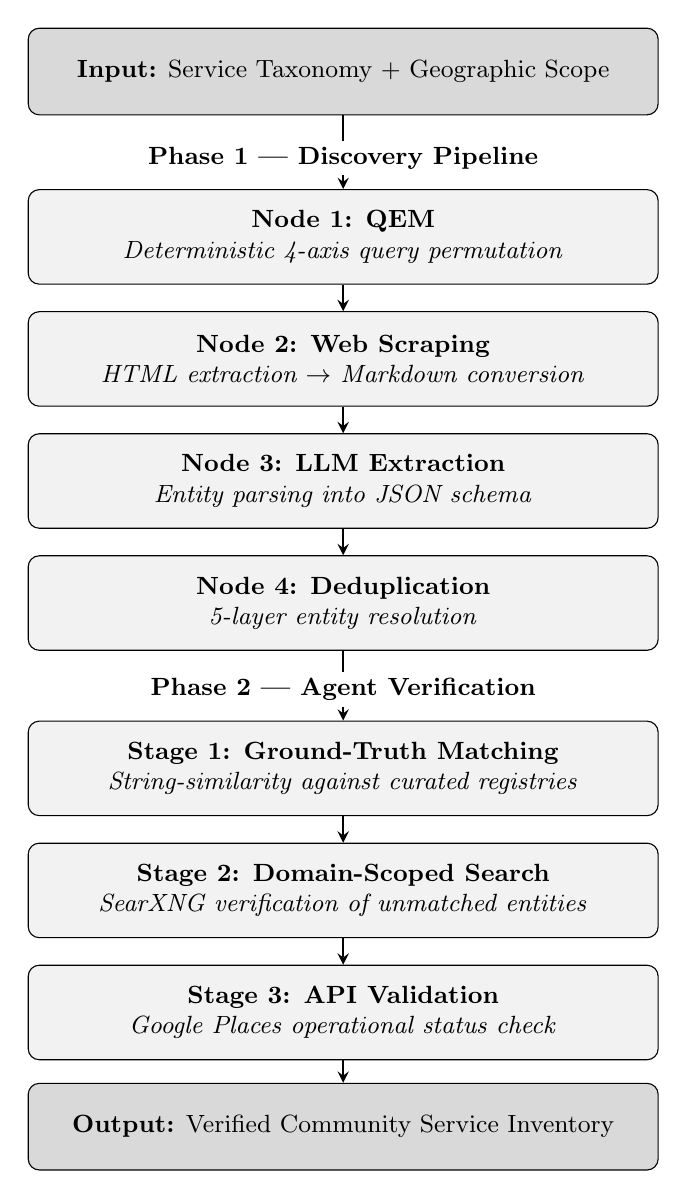
\begin{tikzpicture}[
    node distance=1.55cm,
    process/.style={
        rectangle,
        rounded corners,
        minimum width=8cm,
        minimum height=1.2cm,
        align=center,
        draw=black,
        fill=gray!10,
        font=\small
    },
    iobox/.style={
        rectangle,
        rounded corners,
        minimum width=8cm,
        minimum height=1.1cm,
        align=center,
        draw=black,
        fill=gray!30,
        font=\small
    },
    phlabel/.style={
        font=\small\bfseries,
        align=center,
        draw=none,
        fill=none,
        inner sep=2pt
    },
    arrow/.style={thick, ->, >=stealth}
]

\node (input) [iobox] {\textbf{Input:} Service Taxonomy + Geographic Scope};

\node (ph1) [phlabel, below of=input, node distance=1.1cm] {Phase 1 --- Discovery Pipeline};

\node (n1) [process, below of=ph1, node distance=1.0cm]
    {\textbf{Node 1: QEM} \\ \textit{Deterministic 4-axis query permutation}};
\node (n2) [process, below of=n1]
    {\textbf{Node 2: Web Scraping} \\ \textit{HTML extraction $\rightarrow$ Markdown conversion}};
\node (n3) [process, below of=n2]
    {\textbf{Node 3: LLM Extraction} \\ \textit{Entity parsing into JSON schema}};
\node (n4) [process, below of=n3]
    {\textbf{Node 4: Deduplication} \\ \textit{5-layer entity resolution}};

\node (ph2) [phlabel, below of=n4, node distance=1.1cm] {Phase 2 --- Agent Verification};

\node (s1) [process, below of=ph2, node distance=1.0cm]
    {\textbf{Stage 1: Ground-Truth Matching} \\ \textit{String-similarity against curated registries}};
\node (s2) [process, below of=s1]
    {\textbf{Stage 2: Domain-Scoped Search} \\ \textit{SearXNG verification of unmatched entities}};
\node (s3) [process, below of=s2]
    {\textbf{Stage 3: API Validation} \\ \textit{Google Places operational status check}};

\node (output) [iobox, below of=s3, node distance=1.45cm]
    {\textbf{Output:} Verified Community Service Inventory};

\draw [thick] (input.south) -- (ph1.north);
\draw [arrow] (ph1.south) -- (n1.north);
\draw [arrow] (n1) -- (n2);
\draw [arrow] (n2) -- (n3);
\draw [arrow] (n3) -- (n4);
\draw [thick] (n4.south) -- (ph2.north);
\draw [arrow] (ph2.south) -- (s1.north);
\draw [arrow] (s1) -- (s2);
\draw [arrow] (s2) -- (s3);
\draw [arrow] (s3.south) -- (output.north);

\end{tikzpicture}
\caption{ARS end-to-end pipeline: discovery and agent verification phases.}
\label{fig:ars_system}
\end{figure}

\subsection{Discovery Pipeline}

\textbf{Node 1: Query Expansion Matrix (QEM).} To prevent generative convergence, the QEM enforces structural variance by constructing queries combinatorially across four axes: entity type $e \in \mathcal{E}$, geographic scope $s \in \mathcal{S}$, service attribute $a \in \mathcal{A}$, and source type $t \in \mathcal{T}$. For each four-tuple $(e, s, a, t)$, a deterministic template $\tau$ is selected and the LLM $f_\theta$ is invoked solely to fill the natural-language slots in that template. The model does not choose which queries to issue; it only populates the predetermined structure. This design decouples query diversity from LLM sampling: coverage is a function of the axis cardinalities, not of the model's output distribution. The resulting query set $\mathcal{Q}$ systematically reaches hyper-local domains and non-HTML file types (PDFs, CSVs) that single-shot generation omits.

\vspace{4pt}
\noindent\textbf{Algorithm 1: QEM Traversal}
\begin{algorithmic}[1]
\REQUIRE Entity set $\mathcal{E}$, scope set $\mathcal{S}$, attribute set $\mathcal{A}$, source-type set $\mathcal{T}$, LLM slot-filler $f_\theta$
\ENSURE Query set $\mathcal{Q}$
\STATE $\mathcal{Q} \leftarrow \emptyset$
\FOR{each $e \in \mathcal{E}$}
  \FOR{each $s \in \mathcal{S}$}
    \FOR{each $a \in \mathcal{A}$}
      \FOR{each $t \in \mathcal{T}$}
        \STATE $\tau \leftarrow \textsc{SelectTemplate}(e, s, a, t)$
        \STATE $q \leftarrow f_\theta(\tau,\, e, s, a, t)$ \hfill\COMMENT{LLM fills slots; does not choose queries}
        \STATE $\mathcal{Q} \leftarrow \mathcal{Q} \cup \{q\}$
      \ENDFOR
    \ENDFOR
  \ENDFOR
\ENDFOR
\RETURN $\mathcal{Q}$
\end{algorithmic}
\vspace{4pt}

\textbf{Node 2: Web Scraping and Conversion.} The system programmatically navigates to the URL targets generated in Node 1. The system uses Crawl4AI to extract the raw HTML of each candidate site. To optimize the data for LLM context windows, the unstructured web content is cleaned and converted into standardized Markdown formatting.

The Crawl4AI documentation defines crawl completion through a Boolean success field and exposes the raw HTML, cleaned HTML, Markdown output, links, tables, status code, and error message for inspection \cite{74}. It does not report a universal conversion-accuracy percentage, because content preservation depends on page structure, JavaScript rendering, filtering settings, and the target extraction task. Accordingly, this study reports fetch reliability rather than claiming a vendor accuracy score: in the instrumented addiction-counseling run, 185 of 186 URLs were fetched successfully (99.5\%). Content-level accuracy was assessed downstream through schema extraction, entity verification, and manual review.

\textbf{Node 3: LLM Extraction Engine.} The Markdown documents are divided into processable context chunks. Using strict alignment prompting, the LLM parses the unstructured text into a predefined JSON schema. During this stage, the LLM acts as an active filter, semantically analyzing the text to reject out-of-scope data (e.g., private, for-profit clinics) and retaining only entities that align with the target taxonomy (e.g., public community health services).

\textbf{Node 4: Multi-Layer Deduplication (Entity Resolution).} Because the system scrapes diverse sources, entity overlap is guaranteed. A custom five-layer deduplication pipeline resolves this overlap. \textit{Layer 1 (Hard Match)} applies exact matching on rigid, unique identifiers such as phone numbers. \textit{Layer 2 (Vector Index)} embeds soft identifiers (name and address) into 384-dimensional vectors using the \texttt{all-MiniLM-L6-v2} transformer; entity pairs with cosine similarity above 0.8 are flagged as potential duplicates. \textit{Layer 3 (Hybrid String Math)} subjects flagged pairs to character-level analysis: \texttt{TokenSetRatio} catches word-order shifts and dropped corporate prefixes, while Jaro-Winkler distance handles typographical errors. \textit{Layer 4 (Threshold Routing)} automatically merges pairs scoring above 90\%, separates pairs below 60\%, and routes the 60\%--89\% gray zone to Layer 5. \textit{Layer 5 (LLM Context Judge)} applies an LLM as the final arbiter, using contextual reasoning to disambiguate the remaining gray-zone pairs.

For a local threshold check, we evaluated the deduplication settings on a sample of 200 duplicate and non-duplicate record pairs. We compared the cosine screening values and routing boundaries around the selected configuration. The current configuration (cosine screening at 0.8, automatic merge above 90\%, separation below 60\%, and contextual review in between) produced the best observed balance of duplicate consolidation and preservation of distinct facilities in this sample. This is an engineering validation rather than a domain-wide hyperparameter optimization; broader sensitivity analysis remains future work.

\subsection{Agent Verification Pipeline}

Following deduplication, the ARS applies a three-stage verification pipeline to collect evidence about each extracted entity. These automated signals support triage; final inclusion in the extended ground truth requires manual review.

\textbf{Stage 1: Ground-Truth Matching.} The system attempts to match each extracted entity against domain-appropriate curated registries. To account for LLM formatting variance, the system applies the Layer 3 deduplication algorithm (\texttt{TokenSetRatio} and Jaro-Winkler). Extracted entities achieving high similarity scores against registry records are automatically classified as True Positives.

\textbf{Stage 2: Domain-Scoped Search Verification (SearXNG).} Entities failing Stage 1 are often not hallucinations, but rather valid services absent from the baseline registry due to dynamic web loading or nested pages. The system queries a locally hosted SearXNG instance using targeted search queries (e.g., \texttt{site:<registry-domain> "<entity-name>"}). If a resulting snippet title matches the extracted entity via the string-similarity algorithm, the entity is verified.

\textbf{Stage 3: Real-World API Validation.} Entities failing both Stage 1 and Stage 2 are submitted to the Google Places API via a targeted POST request. Validation relies on two checks: physical existence is confirmed by successfully retrieving a \texttt{place\_id} and an operational \texttt{business\_status}; semantic domain alignment is verified by applying a custom keyword matcher over the API's \texttt{editorialSummary}, \texttt{generativeSummary}, or user \texttt{reviews}. Entities satisfying both criteria are classified as True Positives (Algorithm Discoveries), demonstrating the system's capacity to surface real-world services entirely absent from official, human-curated registries.


\section{Experiments and Evaluation}
\subsection{Experimental Design and Datasets}
We evaluate the ARS across three distinct healthcare service domains, comparing extraction performance against ground truth baselines drawn from curated service directories and independently assembled research datasets.

The evaluation datasets were selected to represent different facets of community care:
\begin{itemize}
    \item \textbf{Addiction Counseling Services:} Sourced from the Ontario 211 database\cite{26}, this dataset acts as a primary benchmark for hyper-local community programs. The objective was to test whether the algorithm could bypass top-level corporate SEO results to extract granular, community-level resources such as mobile outreach units and peer support programs.
    \item \textbf{Hospitals:} Derived from a structured hospital inventory compiled by Kalyani et al. \cite{21} for healthcare entity recognition research, this dataset provides a ground truth of 164 hospital records. This experiment tested the ARS's ability to enumerate large-scale institutional health providers across a regional scope and assess coverage against a systematically assembled reference set.
    \item \textbf{Pharmacy Services:} Drawn from a dataset curated by Ibodeng et al. \cite{22} encompassing Ontario community pharmacy service providers, this dataset offers a ground truth of 404 pharmacy entries. Pharmacy services represent a critical last-mile access point for medication management and chronic disease support, making comprehensive directory coverage particularly valuable for care coordination workflows.
\end{itemize}
\subsection{Evaluation Metrics}
Because traditional curated directories frequently suffer from incomplete coverage, evaluating the generated dataset strictly against a static ground truth would misclassify valid new discoveries as errors. Therefore, we utilize an extended ground truth validation approach.

To measure the SEO Trap operationally, we define the \textit{Popularity Convergence Index} (PCI) for a run as
\[
\mathrm{PCI}=\frac{1}{K}\sum_{k=1}^{K}\frac{|R_k\cap U_k|}{|R_k|},
\]
where $R_k$ is the set of unique entities returned for task $k$, $U_k$ is the subset located in the predefined urban or high-visibility group, and $K$ is the number of evaluated tasks. A complementary \textit{Long-Tail Recovery Rate} (LTRR) is
\[
\mathrm{LTRR}=\frac{1}{K}\sum_{k=1}^{K}\frac{|R_k\cap L_k|}{|L_k|},
\]
where $L_k$ is the independently audited long-tail reference set for task $k$. Higher PCI with lower LTRR indicates concentration in popular locations; lower PCI with higher LTRR indicates broader geographic recovery. In this thesis, the available baseline results are reported descriptively using entity counts and urban/rural distributions. A rigorous future study should repeat each task across models and random seeds and use bootstrap confidence intervals or permutation tests for PCI and LTRR differences.

\subsection{Extended Ground Truth Verification Protocol}

Because community healthcare networks are fundamentally long-tail and subject to rapid operational turnover, static baseline directories often fail to capture the complete regional ecosystem. Consequently, the ARS surfaced a substantial volume of novel entities absent from the GT datasets. To rigorously validate these novel discoveries and prove they were not generative hallucinations, we established an \textit{Extended Ground Truth} via a systematic, manual verification protocol. 

Rather than relying completely on the LLM's internal confidence or isolated API checks, we audited the generated samples using a strict, three-step manual corroboration pipeline:

\begin{enumerate}
    \item \textbf{Independent Source Retrieval:} To avoid validating the ARS against its own potentially flawed extraction paths, each unverified generated entity name and its associated geographic metadata were issued as independent queries through a standard web search engine. 
    \item \textbf{Primary Corroboration:} The resulting search indices were manually reviewed to locate the entity's primary digital footprint independent of the ARS's origin source (e.g., locating an official institutional website, a provincial health registry, or an active social care portal).
    \item \textbf{Semantic and Operational Validation:} Once a primary source was identified, the entity's service profile was manually evaluated against the strict inclusion criteria defined in the initial prompt. The human annotator confirmed that the entity (a) resided strictly within the target geographic boundaries, (b) provided the exact services requested (e.g., dedicated outpatient addiction counseling rather than generalized care), and (c) showed evidence of being currently operational.
\end{enumerate}

Only entities that successfully passed all three stages of this independent auditing process were classified as ``Verified True Positives'' and integrated into the final Extended Ground Truth. This stringent, human-in-the-loop validation step provides evidence that the reported novel discovery rates include genuine community resources rather than consisting entirely of semantic drift or LLM hallucination.

Utilizing this extended GT model, we've defined our evaluation metrics as follows:

\begin{itemize}
    \item \textbf{True Positives (TP):} Any extracted entity that is either (a) successfully matched to a record in the Ground Truth (GT), or (b) programmatically (Section~III) and manually verified as a real, operational institution satisfying the prompt criteria via the ARS agent verification pipeline.
    \item \textbf{False Positives (FP):} Extracted entities that are LLM hallucinations, generic non-entities, or real entities that fall outside the defined prompt constraints.
    \item \textbf{False Negatives (FN):} Valid entities present in the Ground Truth that the algorithm failed to extract. (Note: This metric is inherently skewed by the incomprehensiveness of the GT, serving primarily as a lower-bound indicator for recall).
\end{itemize}

Using these classifications, we calculate \textbf{Precision} (measuring the hallucination rate and prompt adherence), \textbf{Recall} (measuring coverage against the known baseline), and the \textbf{F1-Score} (the harmonic mean of precision and recall).

In this model, Google Places API results were used as corroborating evidence. If an entity was absent from the baseline directory, the API was queried for a valid \texttt{place\_id}, an operational \texttt{business\_status}, and domain-relevant information. Candidates meeting these checks remained subject to the manual audit before inclusion in the extended ground truth.

\subsection{Results and Discussion}
The high-level data collection statistics are summarized by the workflow measurements below, together with the sizes of the ground truth baselines, raw generated extractions, and final deduplicated counts.

\begin{figure}[htbp]
\centering
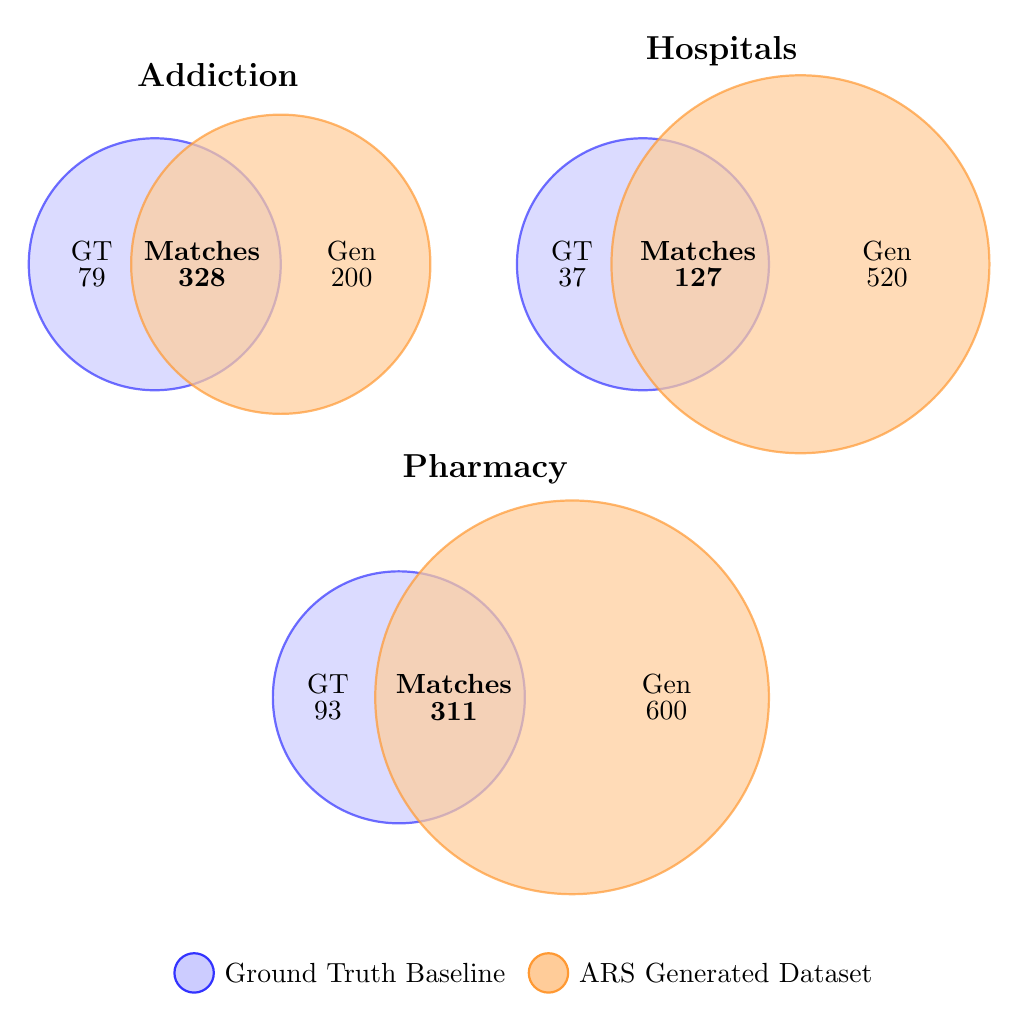
\begin{tikzpicture}[font=\normalsize] 

% 1. Addiction Counseling Diagram (Top Left)
\begin{scope}[shift={(0,0)}]
    \node[circle, draw=blue!80, fill=blue!20, thick, minimum size=3.2cm, opacity=0.7] (GT1) at (0,0) {};
    \node[circle, draw=orange!80, fill=orange!40, thick, minimum size=3.8cm, opacity=0.7] (GEN1) at (1.6,0) {};
    \node at (-0.8, 0) {\shortstack{GT\\79}};
    \node at (0.6, 0) {\shortstack{\textbf{Matches}\\\textbf{328}}};
    \node at (2.5, 0) {\shortstack{Gen\\200}};
    \node[font=\large] at (0.8, 2.4) {\textbf{Addiction}};
\end{scope}

% 2. Hospitals Diagram (Top Right) -- Sized up to prevent text overlap
\begin{scope}[shift={(6.2,0)}] 
    \node[circle, draw=blue!80, fill=blue!20, thick, minimum size=3.2cm, opacity=0.7] (GT2) at (0,0) {};
    \node[circle, draw=orange!80, fill=orange!40, thick, minimum size=4.8cm, opacity=0.7] (GEN2) at (2.0,0) {}; 
    \node at (-0.9, 0) {\shortstack{GT\\37}};
    \node at (0.7, 0) {\shortstack{\textbf{Matches}\\\textbf{127}}};
    \node at (3.1, 0) {\shortstack{Gen\\520}};
    \node[font=\large] at (1.0, 2.7) {\textbf{Hospitals}};
\end{scope}

% 3. Pharmacy Diagram (Bottom Center)
\begin{scope}[shift={(3.1,-5.5)}]
    \node[circle, draw=blue!80, fill=blue!20, thick, minimum size=3.2cm, opacity=0.7] (GT3) at (0,0) {};
    \node[circle, draw=orange!80, fill=orange!40, thick, minimum size=5.0cm, opacity=0.7] (GEN3) at (2.2,0) {}; 
    \node at (-0.9, 0) {\shortstack{GT\\93}};
    \node at (0.7, 0) {\shortstack{\textbf{Matches}\\\textbf{311}}};
    \node at (3.4, 0) {\shortstack{Gen\\600}};
    \node[font=\large] at (1.1, 2.9) {\textbf{Pharmacy}};
\end{scope}

% Unified Legend at the bottom
\begin{scope}[shift={(3.5,-9.0)}]
    \node[circle, fill=blue!20, draw=blue!80, thick, minimum size=0.5cm, label={[font=\normalsize]right:Ground Truth Baseline}] at (-3.0,0) {};
    \node[circle, fill=orange!40, draw=orange!80, thick, minimum size=0.5cm, label={[font=\normalsize]right:ARS Generated Dataset}] at (1.5,0) {};
\end{scope}

\end{tikzpicture}
\caption{Extended Ground Truth Overlap demonstrating the system's high recall (Matches) and massive capacity for novel entity discovery (Gen). Diagram radii are proportional to entity volume, adjusted slightly for text readability.}
\label{fig:venn_diagrams}
\end{figure}

The ARS achieved an average precision of 88.6\% and an average recall of 78.3\% (Table II). These precision scores confirm that the QEM’s structured traversal maintains strict adherence to domain constraints, ensuring the vast majority of extracted entities are valid. The strong recall demonstrates consistent baseline coverage, successfully matching 328 addiction services, 127 hospitals, and 311 pharmacies from the official ground truth.

Crucially, the ARS surfaced a massive volume of verified resources entirely absent from the baseline datasets. These novel discoveries accounted for approximately 61\% of all verified true positives—including 200 addiction services, 520 hospital facilities, and 600 pharmacies. This discovery rate is the direct result of the QEM’s systematic enumeration, proving that structured query architectures successfully reach the long-tail institutional records that traditional generative prompts miss.

Table~\ref{tab:performance_eval} reports the authoritative ARS true-positive, false-positive, and false-negative results. True positives include baseline matches and manually verified discoveries in the extended ground truth. False positives include hallucinated, generic, and out-of-scope extractions. False negatives are valid baseline entities that were not extracted.

\begin{table}[htbp]
\caption{ARS Performance Evaluation}
\label{tab:performance_eval}
\centering
\begin{tabular}{lcccccc}
\toprule
\textbf{Experiment} & \textbf{TP} & \textbf{FP} & \textbf{FN} & \textbf{Precision} & \textbf{Recall} & \textbf{F1-Score} \\
\midrule
Addiction & 528 & 45 & 79 & 92.1\% & 80.6\% & 86.0\% \\
Hospitals & 647 & 154 & 37 & 80.8\% & 77.4\% & 79.1\% \\
Pharmacy & 911 & 71 & 93 & 92.8\% & 77.0\% & 84.1\% \\
\bottomrule
\end{tabular}
\end{table}

\subsubsection{Geographic Distribution and the Long-Tail Fragmentation}
To empirically validate the ARS's ability to bypass generative convergence, the final dataset ($N=2,353$) was stratified geographically. A core objective of this thesis is to prove that the Agentic Research System successfully maps the "long-tail" of community healthcare—the decentralized services that operate outside of densely populated, highly indexed metropolitan hubs. 
\begin{table}[htbp]
\caption{Geographic Distribution of ARS Extracted Entities (Urban vs. Rural)}
\label{tab:ars_geo_distribution}
\centering
\begin{tabular}{lccc}
\toprule
\textbf{Service Domain} & \textbf{Urban Centers} & \textbf{Rural \& Long-Tail} & \textbf{Total Extracted} \\
\midrule
Addiction Counseling & 367 (64.0\%) & 206 (36.0\%) & 573 \\
Hospitals & 347 (40.5\%) & 454 (59.5\%) & 801 \\
Pharmacy Services & 882 (90.1\%) & 97 (9.9\%) & 979 \\
\midrule
\textbf{Total} & \textbf{1,596 (69.8\%)} & \textbf{757 (30.2\%)} & \textbf{2,353} \\
\bottomrule
\end{tabular}
\footnotesize{\textit{Note:} "Urban Centers" denotes high-density municipalities and major Ontario CMAs. "Rural \& Long-Tail" represents decentralized, lower-density townships where traditional SEO indexing is historically weakest.}
\end{table}

The geographic stratification showcased in Table \ref{tab:ars_geo_distribution} reveals the profound capacity of the ARS to bypass traditional indexing blindspots. While the highly commercialized Pharmacy domain naturally clustered in urban centers (90.1\%), the data reveals a completely different reality for critical clinical infrastructure. In the Hospitals and Clinics domain, the ARS discovered significantly more facilities in Rural and Long-Tail regions (59.5\%) than in urban centers. Similarly, the system successfully mapped 206 decentralized Addiction Counseling services operating in the rural data shadow. By enforcing structural variance through the Query Expansion Matrix, the ARS successfully extracts the 639 grassroots entities that exist far beyond the steep drop-off of the urban SEO curve.

Entities were classified into two geographic brackets: high-density urban municipalities and decentralized rural or long-tail municipalities. The aggregate distribution in Table~\ref{tab:ars_geo_distribution} provides the relevant test of geographic coverage without relying on individual-city rankings. Across all domains, 757 of 2,353 geographically classified entities (30.2\%) were in the rural or long-tail bracket. The proportion varied by domain: hospitals had the largest rural share (59.5\%), followed by addiction counseling (36.0\%) and pharmacy services (9.9\%).

This aggregate pattern is consistent with the long-tail hypothesis: resources were recovered outside the most densely populated and highly indexed areas, particularly in the hospital and addiction-counseling domains. It does not establish that every rural service was discovered, nor does it independently prove that the SEO Trap caused the observed distribution. Instead, it provides a reproducible geographic outcome measure that can be compared with the commercial and multi-agent baselines.

\subsubsection{Error Analysis and Boundary Leakage}
While the ARS is highly effective at spidering into these hard-to-reach geographic areas, this aggressive expansion introduces specific failure modes. The recorded false positives (45, 154, 71) were subjected to a proportional analysis across all three domains to better understand the system's limitations.

\begin{figure}[htbp]
\centering
\pgfplotsset{compat=1.18}
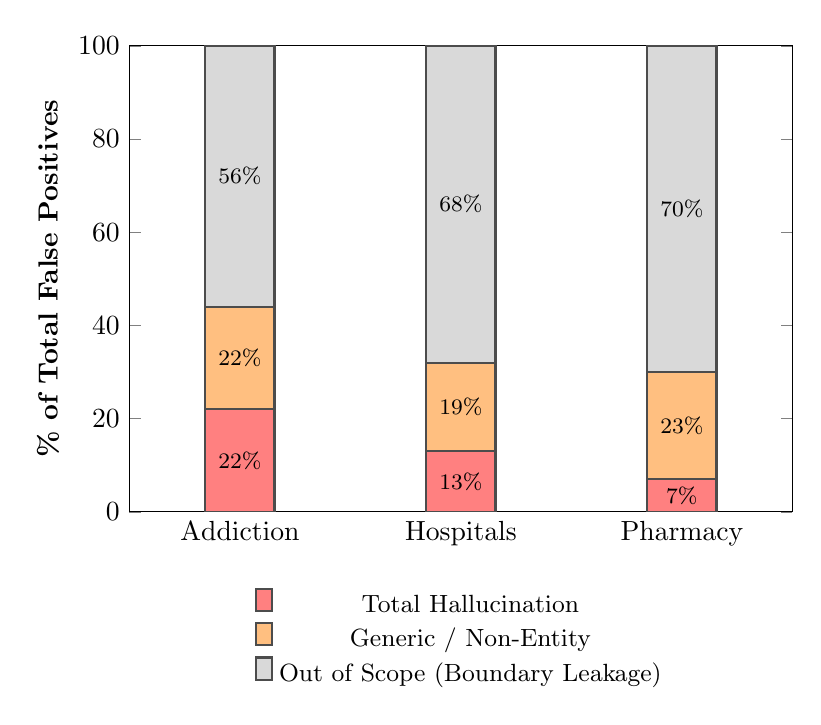
\begin{tikzpicture}
\begin{axis}[
    ybar stacked,
    bar width=25pt,
    width=10cm,
    height=7.5cm,
    ymin=0, ymax=100,
    enlarge x limits=0.25,
    ylabel={\textbf{\% of Total False Positives}},
    symbolic x coords={Addiction, Hospitals, Pharmacy},
    xtick=data,
    y tick label style={font=\normalsize},
    ylabel style={font=\normalsize},
    legend style={
        at={(0.5,-0.15)}, 
        anchor=north, 
        legend columns=1, 
        font=\small,
        draw=none,
        fill=none
    },
    nodes near coords={\pgfmathprintnumber\pgfplotspointmeta\%},
    nodes near coords align={center},
    nodes near coords style={font=\footnotesize, text=black}
]

% 1. Total Hallucination 
\addplot+[ybar, fill=red!50, draw=black!70, thick] plot coordinates {
    (Addiction, 22) (Hospitals, 13) (Pharmacy, 7)
};
% 2. Generic/Non-Entity 
\addplot+[ybar, fill=orange!50, draw=black!70, thick] plot coordinates {
    (Addiction, 22) (Hospitals, 19) (Pharmacy, 23)
};
% 3. Out of Scope
\addplot+[ybar, fill=gray!30, draw=black!70, thick] plot coordinates {
    (Addiction, 56) (Hospitals, 68) (Pharmacy, 70)
};

\legend{Total Hallucination, Generic / Non-Entity, Out of Scope (Boundary Leakage)}
\end{axis}
\end{tikzpicture}
\caption{Error Analysis Breakdown: Proportional distribution of failure modes among False Positives. Note that these percentages represent the breakdown of the erroneous data only, not the entire generated dataset.}
\label{fig:error_breakdown}
\end{figure}

As illustrated in Fig. \ref{fig:error_breakdown}, pure generative hallucinations account for only a small minority of these extraction errors (ranging from 7\% to 22\%). The tertiary verification pipeline effectively mitigates the vast majority of these fabrications. Similarly, generic non-entity extractions remain a secondary issue, largely managed through structured schema enforcement. 

Instead, the primary shortcoming of the current architecture is semantic boundary leakage (Out of Scope extractions). This error mode accounts for the overwhelming majority of False Positives (e.g., 56\% of the errors in Addiction Counseling, and up to 70\% in the Pharmacy dataset). Because community healthcare networks frequently share regional infrastructure, the system's ability to deeply penetrate rural web directories often results in inadvertently pulling in associated facilities from neighboring jurisdictions.

These findings dictate a clear trajectory for future architectural improvements. Because the extraction engine is highly effective at identifying real entities but struggles with geographic drift, future iterations of the ARS must integrate a strict, post-extraction geospatial filtering layer. By cross-referencing extracted postal codes and addresses through a localized Geographic Information System (GIS) or proximity API before the final deduplication stage, the system can aggressively prune out-of-bounds entities. Furthermore, tightening the spatial constraints within the Query Expansion Matrix (QEM) will help restrict the initial search scope, ensuring that the resulting inventory remains strictly hyper-local and immediately actionable for care coordinators.

These results address the care coordination gap outlined in Section I. Under the tested conditions, the ARS achieved 78.3\% baseline recall while also identifying novel verified resources, including resources outside major urban centres. These results support the ARS as a promising inventory-construction workflow, while not establishing province-wide completeness or deployment-scale sustainability.

\subsection{Comparative Evaluation Against Commercial LLMs}
To contextualize the ARS's performance against the current state-of-the-art, we benchmarked our system against three leading commercial generative models: Google's Gemini 1.5 Advanced, OpenAI's ChatGPT Deep Research, and Perplexity AI. The results, summarized in Table~\ref{tab:llm_performance}, provide descriptive evidence consistent with the generative convergence hypothesis.

\begin{table}[htbp]
\caption{Commercial LLM Comparison}
\label{tab:llm_performance}
\centering
\scriptsize
\begin{tabular}{lrrrrrr}
\toprule
\textbf{System} & \textbf{TP} & \textbf{FP} & \textbf{FN} & \textbf{Precision} & \textbf{Recall} & \textbf{F1} \\
\midrule
\multicolumn{7}{l}{\textbf{Hospitals}} \\
ARS & 647 & 154 & 37 & 80.8\% & 77.4\% & 79.1\% \\
Gemini Deep & 224$^{*}$ & 0$^{*}$ & 577$^{*}$ & 100$^{*}$ & 28.0$^{*}$ & 43.8$^{*}$ \\
ChatGPT Deep & 217$^{*}$ & 0$^{*}$ & 584$^{*}$ & 100$^{*}$ & 27.1$^{*}$ & 42.6$^{*}$ \\
Perplexity & $\sim$231$^{*}$ & 0$^{*}$ & $\sim$570$^{*}$ & 100$^{*}$ & 28.8$^{*}$ & 44.8$^{*}$ \\
\multicolumn{7}{l}{\textbf{Addictions}} \\
ARS & 528 & 45 & 79 & 92.1\% & 80.6\% & 86.0\% \\
Gemini Deep & 302$^{*}$ & 0$^{*}$ & 264$^{*}$ & 100$^{*}$ & 53.4$^{*}$ & 69.6$^{*}$ \\
ChatGPT Deep & 38$^{*}$ & 0$^{*}$ & 528$^{*}$ & 100$^{*}$ & 6.7$^{*}$ & 12.6$^{*}$ \\
Perplexity & 222$^{*}$ & 0$^{*}$ & 344$^{*}$ & 100$^{*}$ & 39.2$^{*}$ & 56.3$^{*}$ \\
\multicolumn{7}{l}{\textbf{Pharmacies}} \\
ARS & 911 & 71 & 93 & 92.8\% & 77.0\% & 84.1\% \\
Gemini Deep & 42$^{*}$ & 0$^{*}$ & 937$^{*}$ & 100$^{*}$ & 4.3$^{*}$ & 8.2$^{*}$ \\
ChatGPT Deep & 40$^{*}$ & 0$^{*}$ & 939$^{*}$ & 100$^{*}$ & 4.1$^{*}$ & 7.9$^{*}$ \\
\bottomrule
\end{tabular}
\vspace{2pt}
\footnotesize\parbox{\columnwidth}{\textit{Note:} ARS rows use the independently annotated values in Table~\ref{tab:performance_eval}. Values marked $^{*}$ are optimistic proxies: the reported retrieval count is treated as TP, FP is assumed to be zero, and FN is the difference from the ARS reported count. Precision, recall, and F1 are therefore coverage proxies, not independently annotated metrics. Pharmacy results for systems using a centralized API are excluded.}
\end{table}

\subsubsection{The SEO Trap, Generative Exhaustion, and Geographic Skew}
When tasked with compiling hospital infrastructure, all three commercial baselines fell into an ''SEO Trap.'' Gemini 1.5, ChatGPT, and Perplexity plateaued almost identically between 210 and 224 entities. A qualitative analysis revealed that generative models systematically extract highly indexed, top-level corporate umbrellas while failing to enumerate the localized, physical facilities operating beneath them. 

To quantify this failure, we estimated the geographic distribution of the highest-performing conversational baseline (Gemini) against the ARS, segmented into Urban Centers versus Rural/Long-Tail municipalities (Table \ref{tab:llm_geo_estimate}).

\begin{table}[htbp]
\caption{Estimated Geographic Distribution: Gemini 1.5 vs. ARS}
\label{tab:llm_geo_estimate}
\centering
\begin{tabular}{lcccc}
	oprule
	extbf{Domain} & \multicolumn{2}{c}{\textbf{Urban Centers}} & \multicolumn{2}{c}{\textbf{Rural \& Long-Tail}} \\
\cmidrule(lr){2-3}\cmidrule(lr){4-5}
 & \textit{Gemini} & \textit{ARS (Ours)} & \textit{Gemini} & \textit{ARS (Ours)} \\
\midrule
Hospitals & $\sim$205 & 350 & $\sim$19 & 451 \\
Addictions & $\sim$285 & 360 & $\sim$17 & 206 \\
\bottomrule
\end{tabular}
\end{table}

This geographic stratification reveals that the SEO bias is inherently spatial. Gemini's extraction plateaued entirely within major metropolitan hubs. Without a centralized data source to summarize, conversational models suffer from \textit{Generative Exhaustion}. Once the highly visible urban entities are depleted from their context windows, the models assume the domain is exhausted. In the highly unstructured Addiction Counseling domain, ChatGPT collapsed entirely, yielding only 38 highly indexed, urban treatment centers with \textbf{zero overlap} with the ARS dataset. In contrast, the ARS bypassed this popularity bias to natively map hundreds of hyper-local, decentralized rural facilities.

\subsubsection{The Single-Source Vulnerability}
Perplexity AI's retrieval-augmented architecture yielded distinct, yet equally flawed, behavior. In the Pharmacy domain, Perplexity successfully located and parsed the provincial MOHSERLO database, yielding a massive, province-wide dataset. However, this highlights a critical vulnerability: relying on a "Single Source of Truth." While centralized databases capture high-volume commercial data, they inherently skew toward population density and frequently lack unlisted, grassroots services. 

When Perplexity could not find a neat, pre-compiled dataset for Addiction Counseling, it was forced to scrape the open web. It managed only 221 entities, and strikingly, only 11 of those matched the ARS's footprint. Perplexity captured well-funded, SEO-optimized private rehabilitation centers concentrated in urban hubs, but completely missed the grassroots community networks. Guided by the deterministic Query Expansion Matrix (QEM), the ARS mapped 566 verified facilities, achieving true decentralized discovery across both urban and rural environments.

\subsection{Evaluation of Multi-Agent Systems (MAS) on the Open Web}
Recent literature attempts to automate dataset creation using LLMs but remains constrained by single-shot query generation and human-in-the-loop verification (e.g., Berkane et al. \cite{69}). To determine if explicitly engineered Multi-Agent Systems (MAS) could overcome these limitations autonomously, we evaluated the ARS against InfoSeeker and the AutoData framework \cite{71}, \cite{72} (powered by Browser-Use). 

The empirical results, summarized in Table~\ref{tab:mas_performance}, align with recent large-scale benchmarking studies \cite{73}, revealing that modern MAS architectures function predominantly as fragile ''API scrapers'' rather than robust autonomous discoverers when deployed outside of synthetic environments.

\begin{table}[htbp]
\caption{Multi-Agent System Comparison}
\label{tab:mas_performance}
\centering
\scriptsize
\begin{tabular}{lrrrrrr}
\toprule
\textbf{System} & \textbf{TP} & \textbf{FP} & \textbf{FN} & \textbf{Precision} & \textbf{Recall} & \textbf{F1} \\
\midrule
\multicolumn{7}{l}{\textbf{Hospitals}} \\
ARS & 647 & 154 & 37 & 80.8\% & 77.4\% & 79.1\% \\
InfoSeeker & 231$^{*}$ & 0$^{*}$ & 570$^{*}$ & 100$^{*}$ & 28.8$^{*}$ & 44.8$^{*}$ \\
Browser-Use & 231$^{*}$ & 0$^{*}$ & 570$^{*}$ & 100$^{*}$ & 28.8$^{*}$ & 44.8$^{*}$ \\
\multicolumn{7}{l}{\textbf{Addictions}} \\
ARS & 528 & 45 & 79 & 92.1\% & 80.6\% & 86.0\% \\
InfoSeeker & 33$^{*}$ & 0$^{*}$ & 533$^{*}$ & 100$^{*}$ & 5.8$^{*}$ & 11.0$^{*}$ \\
Browser-Use & 45$^{*}$ & 0$^{*}$ & 521$^{*}$ & 100$^{*}$ & 8.0$^{*}$ & 14.8$^{*}$ \\
\multicolumn{7}{l}{\textbf{Pharmacies}} \\
ARS & 911 & 71 & 93 & 92.8\% & 77.0\% & 84.1\% \\
InfoSeeker & -- & -- & -- & -- & -- & -- \\
Browser-Use & -- & -- & -- & -- & -- & -- \\
\bottomrule
\end{tabular}
\vspace{2pt}
\footnotesize\parbox{\columnwidth}{\textit{Note:} ARS rows use the independently annotated values in Table~\ref{tab:performance_eval}. Values marked $^{*}$ are optimistic proxies: the reported retrieval count is treated as TP, FP is assumed to be zero, and FN is the difference from the ARS reported count. Precision, recall, and F1 are therefore coverage proxies, not independently annotated metrics. Pharmacy systems used a centralized API rather than comparable open-web discovery.}
\end{table}

\subsubsection{The API Scraper Trap and Delegation Failure}
The MAS baselines performed exceptionally well in the Pharmacy domain solely because they successfully attached to the centralized MOHSERLO endpoint. However, relying on a single API inherently adopts the dataset's flaws and regional biases. In the Hospitals domain, both InfoSeeker and Browser-Use defaulted to parsing the same MOHSERLO dataset, hard-plateauing at 231 facilities (the vast majority of which were urban). 

Because this specific dataset lacked phone numbers, the agents attempted to navigate the Ontario College of Pharmacists website for corroboration. Upon encountering a complex JavaScript/UI wall, they failed to extract the target elements. As observed in contemporary evaluations of agentic failure modes, rather than executing a deterministic recovery heuristic, the agents aborted the mission entirely and delegated the task back to a human operator, negating the premise of autonomous discovery.

\subsubsection{Open-Web Crawling Collapse and Pagination Walls}
When deprived of structured APIs and forced to scrape traditional, unstructured web directories, the MAS baselines collapsed entirely. In the highly decentralized Addictions domain, InfoSeeker attempted to scrape the ConnexOntario directory but failed catastrophically on the site's pagination UI, yielding only 33 records. Browser-Use produced roughly 45 samples, severely underperforming compared to the ARS footprint.

\begin{table}[htbp]
\caption{Estimated Geographic Footprint: MAS (InfoSeeker) vs. ARS}
\label{tab:mas_geo_estimate}
\centering
\begin{tabular}{lcccc}
	oprule
\textbf{Domain} & \multicolumn{2}{c||}{\textbf{Urban Centers}} & \multicolumn{2}{c|}{\textbf{Rural \& Long-Tail}} \\
\cmidrule(lr){2-3}\cmidrule(lr){4-5}
 & \textit{InfoSeeker} & \textit{ARS (Ours)} & \textit{InfoSeeker} & \textit{ARS (Ours)} \\
\midrule
Hospitals (API) & $\sim$200 & 350 & $\sim$31 & 451 \\
Addictions (Web) & 33 & 360 & 0 & 206 \\
\bottomrule
\end{tabular}
\footnotesize{\textit{Note:} InfoSeeker's Hospital data reflects the inherent urban skew of the centralized API it scraped, while its Addictions data reflects a complete failure to penetrate the rural web.}
\end{table}

This failure highlights a documented vulnerability in generative navigation: LLM-driven agents frequently struggle to infer state changes (such as \texttt{hasNextPage} triggers) across dynamic JavaScript components and infinite scroll architectures \cite{70}, causing them to prematurely terminate extraction loops. As Table \ref{tab:mas_geo_estimate} illustrates, this UI failure is not geographically neutral. Because web directories typically sort by population density or relevance, failing to navigate past the first page means the MAS captured \textit{only} highly visible urban entities (33), abandoning the entire rural long-tail (0).

These benchmarks support the value of the proposed Query Expansion Matrix (QEM). By specifying a structured query space rather than relying solely on dynamic UI navigation or a single centralized endpoint, ARS provides a reproducible discovery strategy; it does not guarantee exhaustive coverage.

\section{Limitations and Future Work}

While the Agentic Research System (ARS) demonstrates robust capabilities in decentralized healthcare resource mapping, several architectural and environmental limitations constrain its current iteration.

\textbf{The Landing Page Bottleneck and Depth Constraints:} A major limitation of the current extraction pipeline is its reliance on shallow, Depth-0 web scraping. Large community health institutions, such as provincial hospitals, universities, and government ministries, often place their specialized programs, like outpatient vocational rehabilitation, deep in nested sub-directories. Because search engines focus on high-authority root domains, the ARS often retrieves the main landing page instead of the specific program sub-page. As a result, the LLM extraction engine might not recognize the exact healthcare service if it is not clearly outlined on the main index. This requires future integration of agentic, heuristic link-following, or snowball sampling, to navigate institutional site structures on its own.

\textbf{The ``SEO Shadow'' and Query Exhaustion:} The system's capacity to discover hyper-local, community-run health entities is hindered by search engine optimization (SEO) disparities. Small-scale decentralized clinics frequently lack dedicated, high-authority web presence, effectively placing them in an ``SEO shadow'' where they are bypassed by native search engine algorithms in favor of large corporate or government entities. Consequently, querying directly for individual institutions leads to query exhaustion and high data loss. To mitigate this, the current architecture relies on scraping existing regional directories to generate entity candidates prior to verification, which introduces a dependency on the structural integrity of third-party lists. 

\textbf{Computational Cost and API Reliance:} Finally, the framework operates under strict token-economic limits. Running a 1:1 ratio of search queries to individual institutional extractions leads to high LLM API token costs. Additionally, the system's third verification step depends heavily on the Google Places API to confirm the real-world digital footprints of extracted entities. Entities that function legitimately but do not have a registered digital business profile may result in false negatives during verification. This can unintentionally exclude valid community services. Future versions of the ARS should look into lightweight, open-source models for initial extraction to cut down on token usage. They should also consider multi-modal verification systems that do not rely only on proprietary commercial APIs.
\section{Conclusion}
We introduced the Agentic Research System (ARS) for automated discovery and verification of long-tail community health resources on the open web. To overcome \textit{generative convergence} — the tendency of LLM-based query generation to collapse toward high-frequency phrasings and miss low-visibility services — we proposed the Query Expansion Matrix (QEM), a deterministic four-axis enumeration that decouples query diversity from LLM sampling behavior. A three-stage agent verification pipeline programmatically distinguishes real operational entities from hallucinations and scope violations. Evaluated across addiction counseling, hospital, and pharmacy domains, the ARS achieves 88.6\% average precision and 78.3\% average recall against independently validated ground truth baselines, while surfacing approximately 61\% additional verified resources absent from all reference datasets.

Current architectural constraints — Depth-0 web extraction and reliance on the Google Places API for operational verification — limit recovery of services nested in institutional sub-directories or lacking a commercial digital presence. Future work will extend the framework to agentic depth-first crawling and multi-modal verification, advancing autonomous community health resource mapping toward deployment in care coordination workflows.

% % --- Chapter 3 References ---
% \newpage
% \addcontentsline{toc}{section}{References}
% \begin{thebibliography}{99}

% \bibitem{hewner2019improving}
% S. Hewner et al., ``Improving care coordination through community-based health information exchange,'' \textit{Nursing Outlook}, vol. 67, no. 6, pp. 686--696, 2019.

% \bibitem{cartier2020implementing}
% Y. Cartier, C. Fichtenberg, and L. M. Gottlieb, ``Implementing Community Resource Referral Technology: Facilitators and Barriers Described by Early Adopters,'' \textit{Health Affairs}, vol. 39, no. 4, 2020.

% \bibitem{kandpal2023large}
% N. Kandpal et al., ``Large Language Models Struggle to Learn Long-Tail Knowledge,'' in \textit{Proceedings of the International Conference on Machine Learning (ICML)}, 2023.

% \bibitem{berkane2025llm}
% T. Berkane, M.-L. Charpignon, and M. Majumder, ``LLM-Based Web Data Collection for Research Dataset Creation,'' \textit{medRxiv}, 2025.

% \bibitem{yao2023react}
% S. Yao et al., ``ReAct: Synergizing Reasoning and Acting in Language Models,'' in \textit{International Conference on Learning Representations (ICLR)}, 2023.

% \bibitem{zhou2024webarena}
% Y. Zhou et al., ``WebArena: A Realistic Web Environment for Building Autonomous Agents,'' in \textit{International Conference on Learning Representations (ICLR)}, 2024.

% \bibitem{patra2021extracting}
% B. G. Patra et al., ``Extracting social determinants of health from electronic health records using natural language processing: a systematic review,'' \textit{Journal of the American Medical Informatics Association}, vol. 28, no. 12, pp. 2716--2727, 2021.

% \bibitem{gero2023self}
% Z. Gero et al., ``Self-verification improves few-shot clinical information extraction,'' \textit{arXiv preprint arXiv:2306.00024}, 2023.

% \bibitem{peeters2023entity}
% R. Peeters, A. Steiner, and C. Bizer, ``Entity Matching using Large Language Models,'' \textit{arXiv preprint arXiv:2310.11244}, 2023.

% \bibitem{chatgpt} 
% OpenAI, ``Introducing Deep Research,'' \textit{OpenAI Research Blog}, Feb. 2025. [Online]. Available: \url{https://openai.com/index/introducing-deep-research/}

% \bibitem{gemini} 
% Google DeepMind, ``Gemini 1.5: Unlocking multimodal understanding across millions of tokens of context,'' \textit{arXiv preprint arXiv:2403.05530}, 2024.

% \bibitem{claude} 
% Anthropic, ``Developing a computer use model,'' \textit{Anthropic News}, Oct. 2024. [Online]. Available: \url{https://www.anthropic.com/news/developing-computer-use}

% \bibitem{perplexity2025}
% Perplexity AI, ``Perplexity: AI-Powered Search Engine and Research Assistant,'' 2025. [Online]. Available: \url{https://www.perplexity.ai/}

% \bibitem{infoseeker2025}
% AutoData / InfoSeeker Development Team, ``InfoSeeker and Browser-Use: Multi-Agent Systems for Web Information Extraction,'' Evaluation Baseline, 2025.

% \end{thebibliography}
% --- CHAPTER 4 ---
\iffalse
\chapter{Conclusion and Future Work}

This thesis examined whether structured query enumeration can improve the discovery and verification of decentralized community healthcare resources on the open web. The Agentic Research System (ARS) addresses this problem as long-tail retrieval: a small number of highly visible organizations occupy the searchable head, while many valid services are distributed across local pages, institutional sub-pages, PDFs, and directories.

The thesis formalized \textit{Generative Convergence} as the tendency of an LLM-led search process to repeatedly select high-frequency queries and highly visible results, reducing the diversity of discovered entities. The associated ``SEO trap'' is therefore a retrieval and coverage problem, not a claim that search-engine optimization itself is defective. In the experiments, this behavior was assessed descriptively through the geographic distribution and volume of entities returned by commercial generative systems and multi-agent baselines, and through their comparison with ARS output. The evidence is consistent with the hypothesis, but does not establish a causal or universal law.

ARS mitigates this risk with the Query Expansion Matrix (QEM), which enumerates combinations of entity type, geographic scope, service attribute, and source type. The LLM fills slots in predetermined templates rather than deciding the search space. The resulting pages are converted to Markdown, parsed into a structured schema, deduplicated through five layers of entity resolution, and assessed using registry matching, domain-scoped search, and Google Places signals. Manual independent review establishes the extended ground truth for candidates absent from the baseline registries.

Across addiction counseling, hospital, and pharmacy datasets, ARS achieved 88.6\% average precision and 78.3\% average baseline recall. It also identified manually verified resources absent from the baseline inventories. In the workflow sample, 30 query trajectories produced 186 unique URLs; 185 were successfully fetched, 175 source documents yielded 1,148 candidate records, and entity resolution reduced these to 573 deduplicated entities. These measurements characterize one instrumented run and should not be interpreted as province-wide coverage.

The geographic analysis provides an operational definition of long-tail fragmentation for this study. Entities in municipalities with fewer than 100,000 residents were treated as a rural or long-tail bracket. Of 2,353 geographically classified entities, 757 (30.2\%) fell into this bracket, including 454 hospitals (59.5\%) and 206 addiction-counseling services (36.0\%). These descriptive results demonstrate recovery outside major urban centers, but they do not prove that the entire rural ecosystem was found. Comparative baselines also returned fewer entities and smaller estimated rural footprints, although some comparison counts were estimates and some systems used centralized sources.

The findings have several practical implications. First, automated extraction should be frictionless at the system level: the pipeline should handle query construction, fetching, conversion, parsing, and deduplication without requiring an operator to manually navigate every page. This does not mean that evidence assessment is fully automated. Second, the API and search stages are evidence sources rather than definitive arbiters. Third, boundary leakage remains the dominant observed error category, so ARS output should be treated as a research inventory until geographic and programmatic eligibility has been independently validated.

\section{Limitations and Future Work}
The current study has several limitations. The evaluation uses targeted domains and regional datasets rather than the entire province of Ontario. The QEM's query count grows as $|\mathcal{E}|\times|\mathcal{S}|\times|\mathcal{A}|\times|\mathcal{T}|$; province-wide deployment therefore requires hierarchical geographic partitioning, source prioritization, caching, rate limits, and staged scheduling. The practical upper bound cannot be stated from the present experiments because it depends on search quotas, crawl capacity, model cost, and the cardinalities of the four axes.

The study also did not perform a formal ablation or hyperparameter-sensitivity analysis for the 0.8 cosine threshold or the 60\%--90\% routing thresholds. These thresholds should therefore be treated as engineering settings, not optimized universal values. A follow-up study should label candidate pairs across domains and report precision, recall, and F1 over a grid of thresholds, with confidence intervals and a held-out evaluation set.

The comparison with small language models (SLMs) is architectural rather than a head-to-head benchmark. SLMs may require fewer resources and can be effective on bounded, institution-controlled corpora, but they do not by themselves provide a strategy for open-web query enumeration. A fair comparison would hold taxonomy, source set, retrieval budget, and output schema constant, then measure extraction precision, recall, false positives, false negatives, latency, memory, and total cost. The same limitation applies to the commercial and multi-agent comparisons, particularly where centralized APIs or estimated geographic counts were used.

The current crawl is shallow and may miss services buried in nested institutional pages. Future work should evaluate controlled depth-first link following, multimodal processing for scanned PDFs and images, open-source models for lower-cost extraction, and non-proprietary verification sources. A rigorous test of Generative Convergence should randomize tasks and geographic scopes, repeat runs across models and temperatures, and compare query entropy, unique-domain concentration, urban share, rural recall, and overlap with an independently audited reference set. Statistical inference could use bootstrap confidence intervals and mixed-effects or permutation tests over repeated task runs.

Because ARS processes public organizational metadata rather than electronic health records or protected health information, it is designed to reduce privacy exposure. This boundary does not constitute compliance with PHIPA, HIPAA, PIPEDA, OCAP, or national and Indigenous data-sovereignty requirements. Any deployment would require jurisdiction-specific review, data minimization, access control, retention rules, security assessment, provenance policies, and engagement with the communities whose data is represented. Before clinical use, out-of-scope candidates should be quarantined, independently verified against authoritative geographic and program criteria, and excluded from referral workflows unless they meet a documented safety threshold.

\section{Conclusion}
The ARS demonstrates that deterministic query-space construction can complement generative web agents in the discovery of decentralized healthcare resources. The results support improved baseline coverage and recovery of lower-visibility entities, while the remaining uncertainty around causal SEO effects, threshold sensitivity, province-wide scalability, and clinical deployment requires further study. ARS should therefore be understood as an evidence-producing research pipeline and inventory-building system, not as a replacement for authoritative registries or clinical judgment.

\fi

\chapter{Pathways - An Interactive Service-Search and Directory-Maintenance Tool}

\section{Introduction}

The Agentic Research System (ARS) presented in Chapter 3 addresses the cold-start problem of community healthcare discovery. Its results show that a structured discovery pipeline can compile broader candidate inventories under the tested conditions, but they do not establish exhaustive coverage. As established in the literature review, compiling the data only addresses the initial technical bottleneck. A community resource referral system is a complex socio-technical organism. Static healthcare data is incredibly fragile; community clinics frequently alter their hours of operation, SDoH grant funding expires, and intake requirements continuously shift \cite{44, 45, 46}. Without a mechanism for continuous longitudinal maintenance, the AI-generated directory rapidly decays, undermining the clinical trust required for effective care coordination.

Historically, the burden of maintaining these directories has fallen on either centralized administrative teams or the clinical navigators themselves. Relying on healthcare professionals to perform continuous, manual data entry is a fundamentally flawed approach. Extensive literature demonstrates that heavy data-entry tasks are a primary driver of Electronic Health Record (EHR) fatigue and severe burnout among clinicians \cite{53}. Therefore, any viable solution for long-term directory maintenance must be architecturally frictionless, capturing updates without compounding the administrative burden of care coordination.

To solve this longitudinal maintenance challenge, this thesis turns to Human-in-the-Loop (HITL) and crowdsourcing paradigms. Systematic evaluations of crowdsourcing confirm it is a useful methodology for reducing data uncertainty, particularly when the "crowd" consists of domain experts such as discharge planners and social workers \cite{50}. Rather than requiring exhaustive manual overrides, system accuracy may be improved through high-frequency micro-interactions \cite{49, 51}. By capturing repeated, low-friction user feedback, the system may help reduce data drift over time while retaining a role for oversight \cite{54}.

Building on these insights, this chapter introduces \textbf{Pathways}, an interactive service-search and directory-maintenance platform. Pathways bridges the gap between the static ARS extraction pipeline and potential live clinical usage. Operating on a proposed socio-technical flywheel—\textit{Find $\rightarrow$ Verify $\rightarrow$ Ask $\rightarrow$ Close}—the platform integrates human micro-interactions with an immutable, Event-Sourced database architecture \cite{56, 57}. By tying verification events directly to a custom search-ranking algorithm, Pathways creates a mechanism through which verified fields can influence future retrieval. Whether this mechanism produces sustained engagement or clinically adequate directory accuracy requires live evaluation.

\section{Related Works}

The development and evaluation of the Pathways platform intersects with several specialized domains across computer science and health informatics. This section outlines the theoretical and technical precursors to the system, specifically focusing on human-computer interaction (HCI) in clinical AI, immutable data architectures, and the emerging paradigm of agent-based system evaluation.

\subsection{Sociotechnical Collaboration and Trust in Clinical AI}
While autonomous algorithms can process data at unprecedented scales, their integration into clinical workflows frequently fails due to a lack of user trust. Extensive reviews on Human-in-the-Loop (HITL) artificial intelligence in healthcare \cite{48, 51} demonstrate that clinicians are highly hesitant to adopt "black box" systems unless they are provided with mechanisms for collaborative oversight. In high-stakes environments, human operators must feel they have the agency to correct algorithmic assumptions and co-design the system's operational reality \cite{52}. Furthermore, recent scoping reviews on human-AI collaboration emphasize that clinical trust is directly tied to a system's capacity to accept and reflect user feedback \cite{53, 54}.

This HCI principle is foundational to the Pathways architecture. If the Agentic Research System (ARS) from Project 1 operated solely as a static, unalterable directory, navigators would abandon it upon encountering the first outdated clinic profile. By integrating continuous "Verify" and "Flag" micro-interactions directly into the search interface, Pathways transforms the navigator from a passive consumer of AI data into an active collaborator. The system mathematically incorporates their overrides into its ranking logic, thereby natively incentivizing user engagement through immediate, visible system improvement.

\subsection{Data Provenance and Event-Sourced Architectures}
In traditional Create, Read, Update, Delete (CRUD) databases, state changes are destructive; updating a clinic's phone number overwrites the previous value, entirely destroying the historical context of the edit. In healthcare informatics, maintaining an immutable audit trail—data provenance—is highly critical. While alternative cryptographic ledgers are frequently proposed to solve this, they often introduce unnecessary computational overhead for internal clinical software.

Instead, Pathways implements an Event-Sourced Architecture (ESA). As conceptualized by Fowler \cite{55} and standardized in modern data-intensive applications \cite{57}, event-sourced systems store state as an immutable sequence of domain events rather than a table of current values. This real-time, responsive paradigm \cite{60} perfectly serves the crowdsourced flywheel of Pathways. In the proposed data model, a clinic's profile is dynamically derived by folding a chronologically ordered ledger of \texttt{VerificationEvents}. This non-destructive architecture preserves the exact chain of custody for every AI extraction and human correction. Most importantly, it allows the backend to dynamically calculate the temporal "freshness" of any specific data field without relying on a static, easily corrupted timestamp.

\subsection{System Evaluation via Agent-Based Simulation}
Evaluating an interactive, crowdsourced platform traditionally requires long-term deployment with real human cohorts. Because testing the Pathways flywheel on active hospital staff presents significant ethical, privacy, and temporal constraints, this thesis relies on advanced simulated evaluation methodologies. 

The viability of simulation for evaluating human-in-the-loop systems has been explored in computational social science and recommendation research \cite{61,62,64}. However, the present Study 3 does not claim to simulate realistic LLM personas. It uses a deterministic resource model, seeded randomness, controlled verification participation, and a seedable clock to isolate the relationship between participation and freshness decay. This narrower design improves reproducibility but does not estimate how real navigators would behave.

The Pathways system is therefore evaluated through a controlled simulation rather than a synthetic population of AI navigators. Resources begin with known ages, verification events refresh selected resources, and the static control receives no maintenance. This approach tests the mechanics of the proposed flywheel over simulated time while leaving live clinical engagement for future work.

\section{System Architecture and Data Model}
To solve the fragility of traditional healthcare directories, Pathways abandons the standard Create, Read, Update, Delete (CRUD) database paradigm. In a standard CRUD system, state changes are destructive; if a clinic changes its phone number, overwriting the row destroys the historical context of the data. Instead, Pathways is engineered as an Event-Sourced system, conceptually divided into three distinct operational layers: the Ledger, the Projection, and the Interface.

\begin{figure}[htbp]
\centering
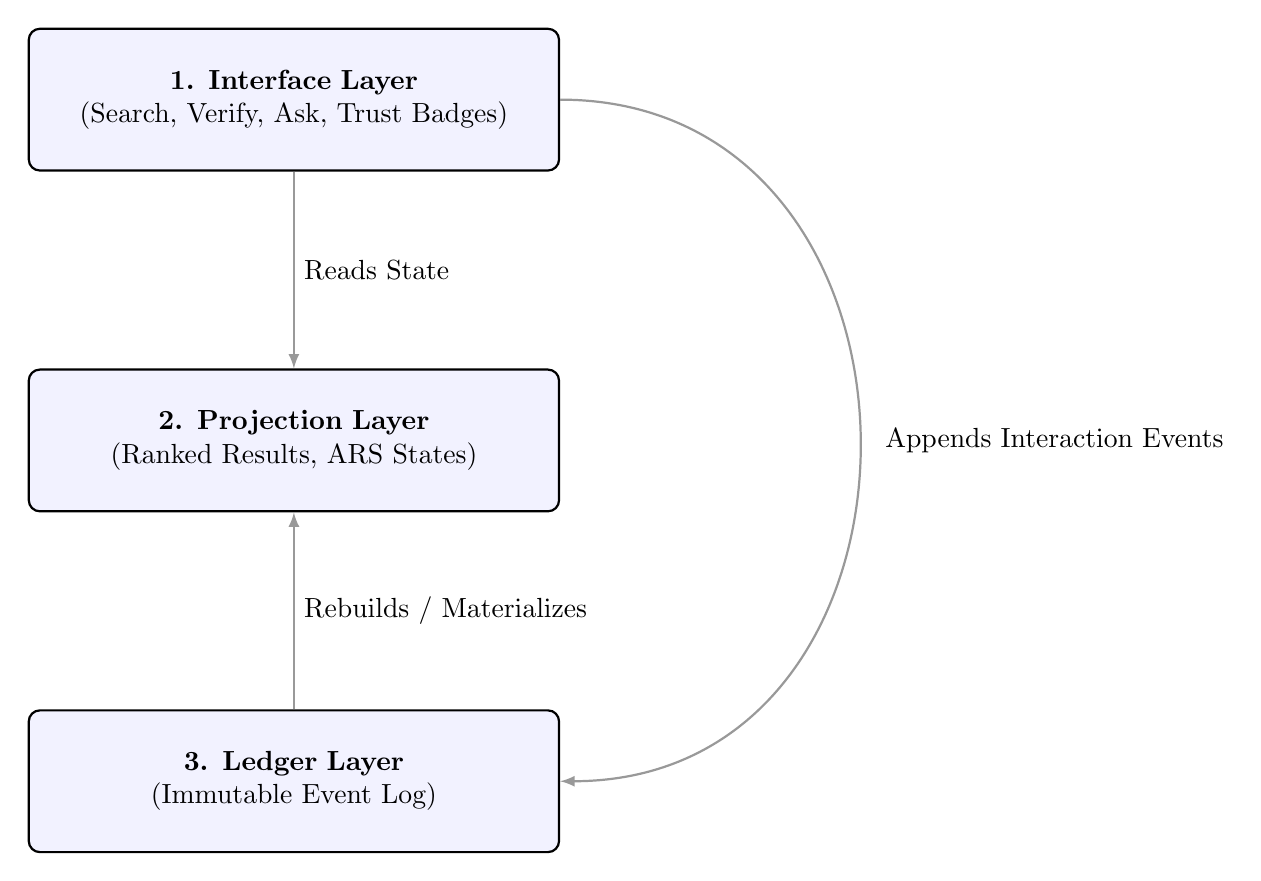
\begin{tikzpicture}[
  node distance=2.5cm and 2cm, 
  auto, thick,
  box/.style={rectangle, draw, fill=blue!5, text width=6.5cm, text centered, minimum height=1.8cm, rounded corners}, 
  arrow/.style={-latex, thick, draw=gray!80} % Swapped to native -latex arrow
]
  
  \node (interface) [box] {\textbf{1. Interface Layer} \\ (Search, Verify, Ask, Trust Badges)};
  \node (projection) [box, below=of interface] {\textbf{2. Projection Layer} \\ (Ranked Results, ARS States)};
  \node (ledger) [box, below=of projection] {\textbf{3. Ledger Layer} \\ (Immutable Event Log)};

  \draw [arrow] (interface.south) -- node[right] {Reads State} (projection.north);
  \draw [arrow] (ledger.north) -- node[right] {Rebuilds / Materializes} (projection.south);
  \draw [arrow] (interface.east) to[out=0, in=0, looseness=1.5] node[right, xshift=0.2cm] {Appends Interaction Events} (ledger.east); 
\end{tikzpicture}
\caption{The Three-Layer Event-Sourced Architecture of Pathways.}
\label{fig:pathways_architecture}
\end{figure}

\subsection{The Three-Layer Architecture}
\begin{itemize}
    \item \textbf{The Ledger (Source of Truth):} The foundational layer is an append-only PostgreSQL database. It stores immutable events such as \texttt{VerificationEvents}, \texttt{AskRequests}, \texttt{ARS\_Replies}, and \texttt{SearchLogs}. The ledger acts as an absolute, auditable chain of custody. 
    \item \textbf{The Projection (Derived State):} The system never queries the ledger directly for front-end rendering. Instead, backend services continuously fold the event ledger to calculate a materialized view—the Projection. This layer contains the field snapshots, pending network suggestions, and the dynamically ranked search results. If a resource's ranking changes, it is strictly because the ranking formula detected a new event in the ledger, not because a data row was manually overwritten.
    \item \textbf{The Interface (Socio-Technical Front-End):} The uppermost layer, prototyped using React and Flask, is the active sensor array. It serves as the point of human-computer interaction, translating clinical searches into a stream of verification and flag events that feed back into the ledger.
\end{itemize}

\section{The Continuous Maintenance Flywheel}
The core operational mechanic of Pathways is a continuous, crowdsourced maintenance flywheel consisting of four sequential phases: \textit{Find, Verify, Ask, and Close}. This loop mathematically aligns human micro-interactions with search engine optimization, inherently rewarding clinical navigators for maintaining the system without inducing Electronic Health Record (EHR) fatigue. 

\subsection{Phase 1: Find (Search and Rank)}
When a navigator queries the system, the Projection layer ranks resources not only by keyword relevance but by data provenance. As demonstrated in Figure \ref{fig:ui_search}, the Pathways search interface provides navigators with immediate visual feedback regarding the algorithm's decision-making process. The UI explicitly separates the semantic \textit{Fit Score} from the \textit{Trust Score} (which represents the temporal freshness decay). This ensures that resources actively verified by the community dynamically bubble to the top of the search index, providing immediate algorithmic transparency to engaged users.

\begin{figure}[H]
    \centering
    \thesisfigure{search_results.png}{0.9\textwidth}
    \caption{The Pathways Search Interface (Phase 1), demonstrating the explicit visual separation of algorithmic Fit Scores and temporal Trust Scores.}
    \label{fig:ui_search}
\end{figure}

The Find phase begins with a filter-extraction layer that translates a navigator's free-text request into the bounded \texttt{SearchFilters} record consumed by the deterministic search adapter. The record contains seven fields: \texttt{need}, \texttt{modality}, \texttt{population}, \texttt{coverage}, \texttt{location}, \texttt{language}, and \texttt{urgency}. Set-valued fields may contain several ontology values, while location and urgency are scalar values. Filter extraction therefore interprets the request; it does not retrieve resources, rank them, or ask the language model to invent a search strategy.

\begin{figure}[htbp]
\centering
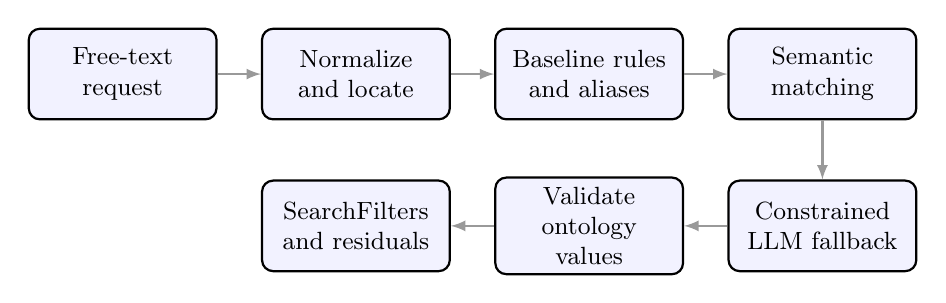
\begin{tikzpicture}[
    node distance=0.75cm and 0.55cm,
    auto, thick,
    stage/.style={rectangle, draw, fill=blue!5, text width=2.15cm, text centered, minimum height=1.15cm, rounded corners, font=\small},
    arrow/.style={-latex, thick, draw=gray!80}
]
    \node (request) [stage] {Free-text\\request};
    \node (normalise) [stage, right=of request] {Normalize\\and locate};
    \node (rules) [stage, right=of normalise] {Baseline rules\\and aliases};
    \node (semantic) [stage, right=of rules] {Semantic\\matching};
    \node (fallback) [stage, below=of semantic] {Constrained\\LLM fallback};
    \node (filters) [stage, left=of fallback] {Validate\\ontology values};
    \node (search) [stage, left=of filters] {SearchFilters\\and residuals};
    \draw [arrow] (request) -- (normalise);
    \draw [arrow] (normalise) -- (rules);
    \draw [arrow] (rules) -- (semantic);
    \draw [arrow] (semantic) -- (fallback);
    \draw [arrow] (fallback) -- (filters);
    \draw [arrow] (filters) -- (search);
\end{tikzpicture}
\caption{Phase 1 filter-extraction pipeline. Deterministic rules and aliases are applied first; semantic matching and the constrained LLM fallback operate only on unresolved or ambiguous residue.}
\label{fig:filter_extraction_pipeline}
\end{figure}

The extraction path is deliberately staged. First, the request is case-folded and separated into known fields; location values are resolved against the resource vocabulary, and empty fields remain explicitly empty. Baseline rules then recognize direct terms and compact patterns such as ``addiction,'' ``walk-in,'' ``same-day,'' and known language or coverage values. The versioned alias map \texttt{hybrid-aliases-v1} extends this coverage with mappings such as ``teenager'' and ``teen'' to \texttt{youth}, ``face-to-face'' to \texttt{in-person}, and ``without OHIP'' to \texttt{no-ohip}.

Unresolved phrases are next ranked against ontology phrase entries using TF-IDF character similarity. Semantic candidates can fill only an empty field and cannot overwrite a deterministic alias. If ambiguity or residual language remains, the optional LLM fallback receives the original query, unresolved terms, the relevant field schema, and the allowed ontology values. It is instructed to return a constrained JSON proposal or abstain. Every proposal is validated against the ontology before merging; the prompt and raw response are retained for audit. The evaluated provider uses the OpenAI-compatible Gemini endpoint.

Finally, unresolved terms are preserved rather than silently converted into unsupported concepts. The resulting structured filters and residual terms are passed to the search adapter, which applies fit and freshness scoring over the normalized resource corpus. This separation keeps filter interpretation, retrieval, ranking, and provenance as distinct responsibilities.

\begin{table}[H]
\caption{Pathways filter-extraction stages and responsibilities}
\label{tab:filter_extraction_stages}
\centering
\scriptsize
\begin{tabularx}{\textwidth}{@{}p{2.0cm}X p{3.0cm} p{2.7cm}@{}}
\toprule
\textbf{Stage} & \textbf{Operation} & \textbf{Evidence recorded} & \textbf{Current condition} \\
\midrule
Normalization & Case-folding, field separation, and location lookup. & Input query and structured field candidates. & Deterministic \\
Baseline rules & Direct vocabulary and regular-expression matches. & Field values and mismatches. & Implemented and evaluated \\
Ontology aliases & Maps paraphrases to existing ontology values. & Alias phrase, field, concept, and ontology version. & Implemented as development hybrid \\
Semantic matching & TF-IDF character-similarity ranking against ontology phrase entries. & Candidate phrase, concept, and similarity score. & Implemented and ablated \\
LLM fallback & Proposes constrained ontology values for unresolved or ambiguous phrases. & Prompt, proposal, model, and raw response. & Implemented with Gemini \\
Open-world residuals & Retains unresolved terms rather than forcing a filter. & Residual terms and extraction route. & Trace signal implemented \\
\bottomrule
\end{tabularx}
\end{table}

\subsection{Phase 2: Verify (Frictionless Validation)}
If the navigator successfully utilizes a resource, they transition to the validation phase. As shown in Figure \ref{fig:ui_verify}, the resource detail card is engineered for frictionless micro-interactions. Next to high-decay data fields—such as Phone Numbers, Websites, and Operating Hours—the interface features dedicated ``Verify'' and ``Flag Issue'' buttons. Utilizing an optimistic UI architecture, clicking Verify immediately registers the validated state locally (turning the badge green) to prevent cognitive interruption, while asynchronously appending a \texttt{VerificationEvent} to the backend ledger. This action instantly resets the resource's freshness decay curve to $1.0$.

\begin{figure}[H]
    \centering
    \thesisfigure{verify.png}{0.95\textwidth}
    \caption{The Resource Detail Interface (Phase 2), featuring inline, zero-friction verification and flagging controls for highly mutable data fields.}
    \label{fig:ui_verify}
\end{figure}

\subsection{Phase 3: Ask (Flagging and ARS Integration)}
If a navigator encounters stale data, they click the inline ``Flag Issue'' button rather than abandoning the resource entirely. This appends a flag event to the ledger, which immediately routes the stale resource into the system's asynchronous ``Ask'' queue. Crucially, as depicted in Figure \ref{fig:ui_ask_queue}, this queue bridges the human interface with the Agentic Research System (ARS) developed in Project 1. The ARS functions as a background worker monitoring the \texttt{ARS\_ENRICHING} state. When triggered, it automatically scans the open web for updated contact information without requiring the clinical navigator to manually research the missing data.

\begin{figure}[H]
    \centering
    \thesisfigure{ask_ars_job_queue.png}{0.9\textwidth}
    \caption{The Ask Board and ARS Job Queue (Phase 3), illustrating the asynchronous delegation of flagged resources to the autonomous AI background worker.}
    \label{fig:ui_ask_queue}
\end{figure}

\subsection{Phase 4: Close (Human-AI Resolution)}
In the final phase of the socio-technical loop, a human operator reviews the ARS's cached discoveries. Figure \ref{fig:ui_close} demonstrates the resolution interface, which explicitly compares the ``Old Value'' against what the ``ARS Found.'' If the ARS correctly identified the new clinic hours or web address, the human clicks ``Accept Suggestion.'' This one-click resolution triggers a closing event in the ledger, which seamlessly updates the Projection layer, restores the resource's Trust Score, and completes the maintenance flywheel. 

\begin{figure}[H]
    \centering
    \thesisfigure{Ask_results.png}{0.7\textwidth}
    \caption{The Resolution Interface (Phase 4), enabling human operators to seamlessly validate and accept the ARS's autonomously discovered data updates.}
    \label{fig:ui_close}
\end{figure}

\begin{figure}[htbp]
\centering
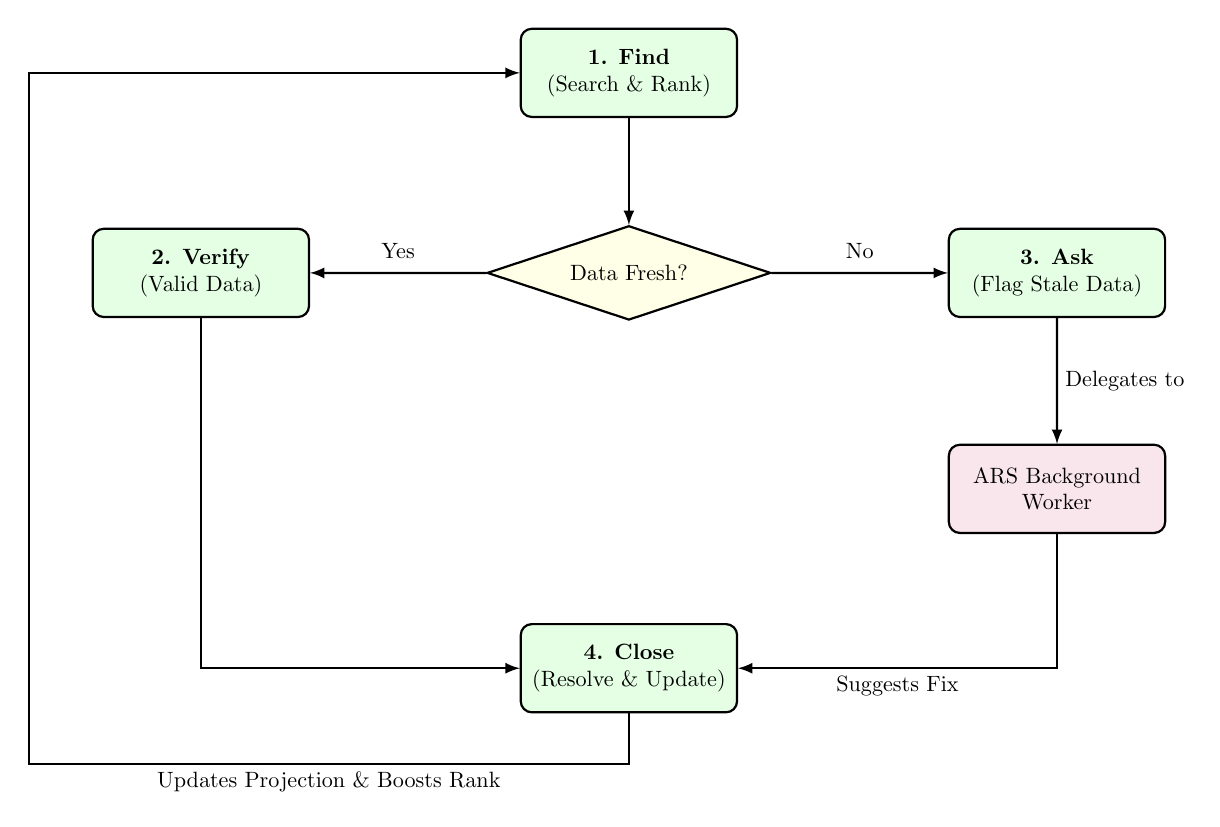
\begin{tikzpicture}[
    scale=0.80, transform shape,
    node distance=2cm and 2cm,
    auto, thick,
    process/.style={rectangle, draw, fill=green!10, text width=3.2cm, text centered, minimum height=1.4cm, rounded corners},
    decision/.style={diamond, aspect=2, draw, fill=yellow!10, text centered, minimum width=4.5cm, inner sep=3pt},
    ars/.style={rectangle, draw, fill=purple!10, text width=3.2cm, text centered, minimum height=1.4cm, rounded corners},
    arrow/.style={-latex, thick}
]
    \node (find) [process] {\textbf{1. Find} \\ (Search \& Rank)};
    \node (eval) [decision, below=of find, yshift=0.3cm] {Data Fresh?};
    \node (verify) [process, left=of eval, xshift=-0.8cm] {\textbf{2. Verify} \\ (Valid Data)};
    \node (flag) [process, right=of eval, xshift=0.8cm] {\textbf{3. Ask} \\ (Flag Stale Data)};
    \node (arsnode) [ars, below=of flag] {ARS Background \\ Worker};
    \node (close) [process, below=of eval, yshift=-2.8cm] {\textbf{4. Close} \\ (Resolve \& Update)};
    \draw [arrow] (find.south) -- (eval.north);
    \draw [arrow] (eval.west) -- node[above, yshift=0.1cm] {Yes} (verify.east);
    \draw [arrow] (eval.east) -- node[above, yshift=0.1cm] {No} (flag.west);
    \draw [arrow] (flag.south) -- node[right] {Delegates to} (arsnode.north);
    \draw [arrow] (arsnode) |- node[below, pos=0.75] {Suggests Fix} (close.east);
    \draw [arrow] (verify) |- (close.west);
    \draw [arrow] (close.south) -- ++(0,-0.8cm) -| node[pos=0.25, below] {Updates Projection \& Boosts Rank} ([xshift=-1.0cm]verify.west) |- (find.west);
\end{tikzpicture}
\caption{The socio-technical flywheel integrating human validation with the ARS background worker.}
\label{fig:core_loop}
\end{figure}


\section{Validation and Simulation Methodology}
Evaluating an interactive, crowdsourced platform traditionally requires long-term deployment across active clinical cohorts. Because deploying an experimental prototype in a live hospital setting presents significant privacy and temporal constraints, this thesis evaluates Pathways through complementary offline studies covering request interpretation, ranking quality, simulated freshness maintenance, and targeted restoration. Interface telemetry and live clinical engagement remain future work.

\subsection{Study 1: Natural-language filter extraction}
Study 1 evaluates whether ordinary requests can be converted into the structured filters used by Pathways search. The fixture contains 200 structured queries generated from ten filter families crossed with ten Ontario locations, with 100 canonical and 100 paraphrased queries. Gold labels cover need, modality, population, coverage, location, language, and urgency. We report exact-case accuracy, field-level exact accuracy, and micro-averaged precision, recall, and F1.

The primary comparison is between the deterministic baseline, the alias-enhanced hybrid extractor, and the optional semantic and constrained-fallback stages. The evaluator records the gold filter, system output, field-level matches, residual terms, extraction route, and LLM provenance for every query. Exact-case accuracy is strict: all seven fields must agree for a query to count as correct. This separation is important for interpreting the result because Study 1 measures request interpretation, not end-to-end retrieval quality.

The real-provider condition used the OpenAI-compatible Gemini endpoint configured through \texttt{GEMINI\_API\_KEY} and \texttt{GEMINI\_MODEL}. The fallback was constrained to ontology values and could abstain; it was not allowed to invent new filter concepts. The resulting report is retained as \texttt{study1\_semantic\_llm\_gemini\_report.json}.

Table~\ref{tab:filter_extraction_stages} is located in the System Architecture section because it describes implementation responsibilities rather than an experimental result.

\subsection{Study 2: Information retrieval quality}
Study 2 evaluates ranking quality on eight cases and twelve resources using 96 independently adjudicated graded relevance judgments. Pathways is compared with a fit-only variant and a local BM25 implementation using Precision@5, graded nDCG@5, mean reciprocal rank, and mean average precision. The adjudicated set is treated as the primary result; earlier hand-authored development labels are reported only as calibration evidence.

\subsection{Study 3: Simulated flywheel maintenance}
Study 3 evaluates whether verification participation counteracts freshness decay. A deterministic simulator compares an unmaintained static directory with a flywheel condition at $T=0$, $30$, and $90$ days. Verification participation is swept from 0\% to 100\% in 25\% increments, with ten seeds per condition. This is simulated longitudinal evidence rather than observation from a 90-day clinical deployment.
\subsection{Study 4: Targeted missing-data restoration}
Study 4 evaluates Pathways Data Restoration on a sealed 500-field benchmark. The workflow combines entity-supported Places results with the ARS fallback for unresolved cases. We report requested fields by category and classify each result as exact, supported but non-exact, weakly supported, or unresolved after manual review.

\subsection{Evaluation results}
Table~\ref{tab:pathways_study_summary} summarizes the completed studies. The extraction and ranking experiments use different targets: Study 1 measures structured interpretation of requests, while Study 2 measures ordering of candidate resources. Study 3 tests the maintenance mechanism under controlled simulated time, and Study 4 measures evidence-backed recovery of missing fields.

% \subsubsection{How to interpret the evaluation measures}
The four studies answer different questions and should not be collapsed into a single accuracy number. Study 1 asks whether a request is translated into the intended structured filters. Study 2 asks whether relevant resources appear near the top of a ranked list. Study 3 asks whether a specified verification process can counteract simulated freshness decay. Study 4 asks whether a missing organizational field can be restored with evidence that belongs to the intended organization.

For Study 1, \textit{precision} is the proportion of extracted filter values that are correct, \textit{recall} is the proportion of gold filter values that were extracted, and F1 is their harmonic mean. Exact-case accuracy is stricter: every field for a query must match the gold record for the query to count as correct. For Study 2, Precision@5 measures the fraction of the first five results that are relevant, while nDCG@5 additionally rewards putting highly relevant resources above merely relevant ones. MRR records the reciprocal rank of the first relevant result, and MAP averages precision at the ranks where relevant results occur. For Study 3, a resource is counted as fresh when its simulated freshness score is at least 0.75 and stale when it is below 0.25. For Study 4, a \textit{filled} field is non-empty, an \textit{entity-supported} field has sufficient agreement between the candidate and the target organization, and an \textit{exact} field matches the sealed reference after field normalization.

The Study 4 entity-support check combines available identity evidence such as name, city, address, postal code, and website domain. It is deliberately stricter than checking whether a returned value merely looks plausible. Consequently, a supported value may be non-exact because an organization has changed its website or because the same value has a different representation. Conversely, a value classified as unsupported should be treated as unsafe for automatic acceptance, even when it appears superficially reasonable. In this thesis, ``wrong entity'' means ``failed the entity-support threshold''; it is not a claim that every such case was manually proven to belong to a different organization.

The same principle applies across the other studies: each metric is tied to a defined decision. Study 1 correctly maps the canonical query ``youth mental health Scarborough'' to the population filter ``youth''. In the hybrid condition, the paraphrase ``mental health help for a teenager in Scarborough'' is also mapped to the ontology's ``youth'' value, although the fixture distinguishes ``youth'' from ``adolescent'' in three cases. This is an ontology-alignment issue rather than a ranking failure. In Study 2, a result can be relevant without being the highest-graded result; nDCG distinguishes those ordering differences even when MRR remains perfect. In Study 3, a day-90 fresh rate of 0.50 means that half of the simulated resources satisfy the freshness threshold at that time point; it is not a percentage of real users or a clinical success probability.

\begin{table}[H]
\caption{Worked interpretation examples across Studies 1--3}
\label{tab:cross_study_examples}
\centering
\scriptsize
\begin{tabularx}{\textwidth}{@{}p{1.4cm}p{3.0cm}X X@{}}
\toprule
\textbf{Study} & \textbf{Input} & \textbf{Observed output} & \textbf{What the result means} \\
\midrule
1 & ``youth mental health Scarborough'' & Population = youth; location = Scarborough & Exact extraction on a canonical vocabulary case \\
1 & ``mental health help for a teenager in Scarborough'' & Hybrid maps teenager to population = youth & Alias coverage improves interpretation; exact ontology alignment still matters \\
2 & ``Mandarin home care Scarborough'' & Pathways ranks Yee Hong first; BM25 ranks Spectrum first & Both return relevant candidates; nDCG evaluates the graded ordering \\
3 & 50\% participation at day 90 & Mean fresh rate = 0.50 across ten seeds & Half of simulated resources meet the freshness threshold; not a real-world adoption rate \\
\bottomrule
\end{tabularx}
\end{table}

\begin{table}[H]
\caption{Summary of Pathways evaluation studies}
\label{tab:pathways_study_summary}
\centering
\small
\begin{tabularx}{\textwidth}{@{}p{1.1cm}X p{3.2cm} p{2.5cm}@{}}
\toprule
\textbf{Study} & \textbf{Evaluation target} & \textbf{Dataset or conditions} & \textbf{Primary result} \\
\midrule
1 & Natural-language filter extraction & 200 queries; 100 canonical and 100 paraphrased & Basic F1 $=0.892$; semantic + Gemini F1 $=1.000$, exact $=1.000$ \\
2 & Ranked retrieval quality & 8 cases, 12 resources, 96 adjudicated judgments & BM25 nDCG@5 $=0.916$; Pathways $=0.804$ \\
3 & Freshness maintenance & 0--100\% participation; 10 seeds; $T=0,30,90$ days & Day-90 fresh rate: $0.00$ to $1.00$ \\
4 & Missing-data restoration & 500 requested fields; Places plus ARS fallback & 142 exact; 284 supported non-exact; 63 weak; 11 unresolved \\
\bottomrule
\end{tabularx}
\end{table}

\subsubsection{Study 1 results}
The structured 200-query fixture was generated from ten filter families crossed with ten Ontario
locations. Each family contributes one canonical and one paraphrased query,
yielding 100 queries in each category. The five conditions isolate the
contributions of basic rules, ontology aliases, semantic matching, Gemini
alone, and semantic matching combined with Gemini.

\begin{table}[H]
\caption{Expanded Study 1 five-condition results}
\label{tab:study1_expanded_results}
\centering
\small
\begin{tabular}{lrrrr}
\toprule
\textbf{Condition} & \textbf{Overall exact} & \textbf{Canonical exact} & \textbf{Paraphrased exact} & \textbf{Micro-F1} \\
\midrule
Basic rules & 0.600 & 1.000 & 0.200 & 0.8916 \\
Hybrid aliases & 0.750 & 1.000 & 0.500 & 0.9318 \\
Semantic-only & 0.900 & 1.000 & 0.800 & 0.9663 \\
Gemini-only & 0.950 & 1.000 & 0.900 & 0.9890 \\
Semantic + Gemini & 1.000 & 1.000 & 1.000 & 1.0000 \\
\bottomrule
\end{tabular}
\end{table}

\begin{figure}[H]
\centering
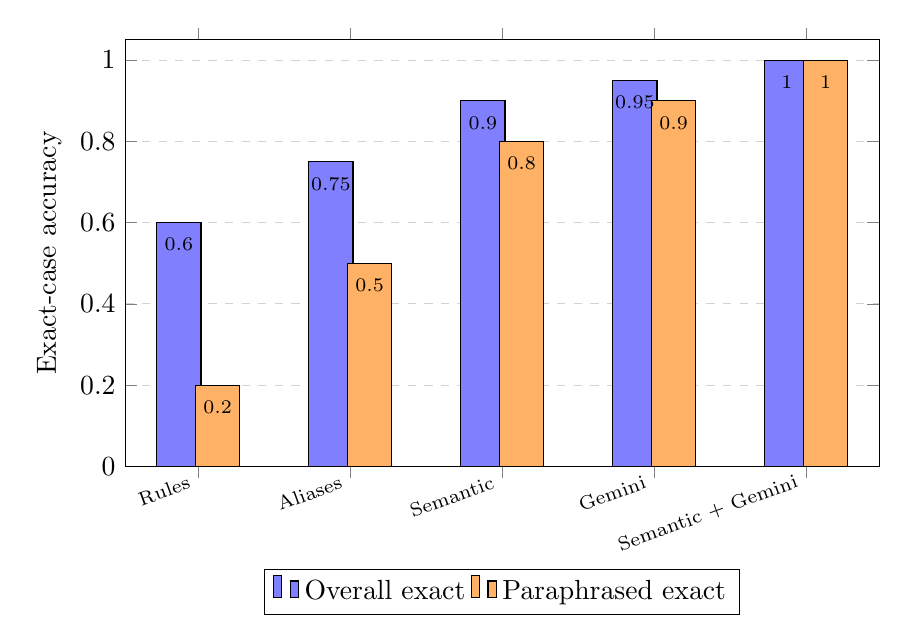
\begin{tikzpicture}
\begin{axis}[
    ybar,
    bar width=16pt,
    width=0.92\textwidth,
    height=7cm,
    ymin=0,
    ymax=1.05,
    ylabel={Exact-case accuracy},
    symbolic x coords={Rules,Aliases,Semantic,Gemini,Semantic+Gemini},
    xtick=data,
    xticklabels={Rules,Aliases,Semantic,Gemini,Semantic + Gemini},
    x tick label style={font=\scriptsize, rotate=20, anchor=east},
    nodes near coords,
    nodes near coords align={center},
    nodes near coords style={font=\scriptsize, text=black, yshift=-8pt},
    enlarge x limits=0.12,
    ymajorgrids=true,
    grid style={dashed,gray!35},
    legend style={at={(0.5,-0.24)},anchor=north,legend columns=2}
]
\addplot[fill=blue!50, bar shift=-7pt] coordinates {
    (Rules,0.600) (Aliases,0.750) (Semantic,0.900) (Gemini,0.950) (Semantic+Gemini,1.000)
};
\addlegendentry{Overall exact}
\addplot[fill=orange!60, bar shift=7pt] coordinates {
    (Rules,0.200) (Aliases,0.500) (Semantic,0.800) (Gemini,0.900) (Semantic+Gemini,1.000)
};
\addlegendentry{Paraphrased exact}
\end{axis}
\end{tikzpicture}
\caption{Expanded Study 1 exact-case accuracy across the five extraction conditions. Values are development-fixture results; labels are placed inside the bars.}
\label{fig:study1_expanded_accuracy}
\end{figure}

The structured benchmark shows a clear progression on paraphrased requests.
Basic rules achieved 0.200 paraphrase exact accuracy, aliases increased this
to 0.500, and semantic-only matching increased it to 0.800. Gemini-only
reached 0.900, while the combined semantic-plus-Gemini condition reached
1.000 on this fixture. The Gemini conditions were evaluated using four
batched requests of 50 cases. Because the fixture and ontology were used
during implementation, these results are development evidence rather than
held-out estimates of general language understanding.

\subsubsection{Study 2 results}
On the independently adjudicated relevance set, all three methods retrieved at least one relevant result at the top of the ranking, producing MRR and MAP of 1.00. The more discriminating graded metric favored BM25: nDCG@5 was 0.916 for BM25, 0.879 for the fit-only variant, and 0.804 for Pathways. Precision@5 was 1.00 for all three methods on this small set. Thus, the current Pathways ranking demonstrates strong early retrieval but does not outperform lexical BM25 on graded ordering. This is a limitation of the current fit--freshness weighting, not evidence that provenance and freshness are unhelpful objectives.

\begin{table}[H]
\caption{Study 2 independently adjudicated ranking results}
\label{tab:study2_results}
\centering
\small
\begin{tabular}{lrrrr}
\toprule
\textbf{Ranker} & \textbf{Precision@5} & \textbf{nDCG@5} & \textbf{MRR} & \textbf{MAP} \\
\midrule
Pathways & 1.000 & 0.804 & 1.000 & 1.000 \\
Fit-only & 1.000 & 0.879 & 1.000 & 1.000 \\
BM25 & 1.000 & 0.916 & 1.000 & 1.000 \\
\bottomrule
\end{tabular}
\end{table}

\subsubsection{Study 3 results}
The deterministic sweep produced a monotonic relationship between participation and day-90 freshness. With no verification participation, the flywheel condition behaved like the static control: mean fresh rate was 0.00 and mean stale rate was 1.00. At 50\% participation, mean fresh rate was 0.50 and mean stale rate was 0.50. At full participation, all simulated resources were fresh at day 90. The 25\%, 50\%, and 75\% conditions had fresh-rate standard deviations of 0.156, 0.161, and 0.140 across ten seeds. These results support the mechanism under the simulator's assumptions, but they do not estimate real navigator participation or prove clinical self-maintenance.

\begin{figure}[H]
\centering
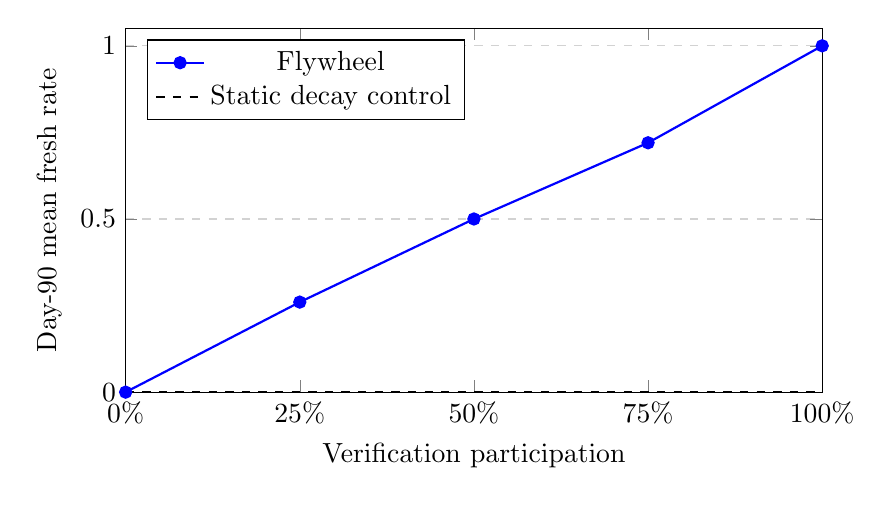
\begin{tikzpicture}
\begin{axis}[
    width=0.86\textwidth, height=6.2cm,
    xlabel={Verification participation}, ylabel={Day-90 mean fresh rate},
    xmin=0, xmax=1, ymin=0, ymax=1.05,
    xtick={0,0.25,0.5,0.75,1}, xticklabels={0\%,25\%,50\%,75\%,100\%},
    ymajorgrids=true, grid style={dashed,gray!35}, legend pos=north west
]
\addplot[mark=*, thick, blue] coordinates {(0,0) (0.25,0.26) (0.5,0.50) (0.75,0.72) (1,1.00)};
\addlegendentry{Flywheel}
\addplot[dashed, thick, black] coordinates {(0,0) (1,0)};
\addlegendentry{Static decay control}
\end{axis}
\end{tikzpicture}
\caption{Study 3 simulated day-90 freshness as verification participation increases.}
\label{fig:study3_participation}
\end{figure}

\subsubsection{Study 4 results}
The Pathways Data Restoration condition requested 500 missing fields. After manual review, 142 values were exact, 284 were supported but non-exact, 63 were weakly supported, and 11 were unresolved. The categories are intentionally separate: exact values match the sealed reference; supported non-exact values are accepted alternate representations, including departmental phone numbers and alternate website representations; weakly supported values are plausible but require further confirmation; unresolved cases produced no acceptable value. The result supports Pathways as an assistive restoration workflow, not as an autonomous source of truth.

Table~\ref{tab:study4_examples} gives concrete examples from the benchmark. In the first example, the input record is missing only a postal code. Pathways returns ``M4L 2A4'', which agrees exactly with the sealed reference and is supported by the matching pharmacy name and address. In the second example, the requested website differs from the stored reference: the reference contains a directory URL, while Pathways returns the pharmacy's organizational website. The value is supported but non-exact, illustrating why exact and supported categories are reported separately. In the third example, the system returns no phone number; this is unresolved. The final example is weakly supported because the returned address is plausible for the named pharmacy but does not match the expected unit-level representation. Such values require manual review rather than automatic acceptance.

\begin{table}[H]
\caption{Worked examples of Study 4 field outcomes}
\label{tab:study4_examples}
\centering
\scriptsize
\begin{tabularx}{\textwidth}{@{}p{1.5cm}p{2.6cm}X X p{1.7cm}@{}}
\toprule
\textbf{Outcome} & \textbf{Target and missing field} & \textbf{Sealed reference} & \textbf{System output} & \textbf{Interpretation} \\
\midrule
Exact & L \& A Pharmacy; postal code & M4L 2A4 & M4L 2A4, supported by matching name, address, and city & Filled; supported; exact \\
Supported, non-exact & Main and Bronte Pharmacy; website & Healthline directory URL & Pharmacy organizational website; same named organization and address & Filled; supported; not exact \\
Unresolved & Humber River Health; phone & 416-242-1000 & No phone value returned & No fill; requires review or another source \\
Weakly supported baseline & Main Drug Mart; address & 1 Oak St, Units 1--2 & 1 Oak St, Toronto, ON M5A 0A1 & Plausible-looking value, but not automatically accepted without sufficient support \\
\bottomrule
\end{tabularx}
\end{table}

\begin{table}[H]
\caption{Study 4 Pathways Data Restoration results by missing-field category}
\label{tab:study4_results}
\centering
\small
\begin{tabular}{lrrrrr}
\toprule
\textbf{Missing field} & \textbf{Requested} & \textbf{Exact} & \textbf{Supported, non-exact} & \textbf{Weakly supported} & \textbf{Unresolved} \\
\midrule
Address & 269 & 11 & 201 & 57 & 0 \\
Phone number & 112 & 77 & 34 & 0 & 1 \\
Postal code & 58 & 52 & 0 & 6 & 0 \\
Website & 61 & 2 & 49 & 0 & 10 \\
\textbf{Total} & \textbf{500} & \textbf{142} & \textbf{284} & \textbf{63} & \textbf{11} \\
\bottomrule
\end{tabular}
\end{table}

% --- CHAPTER 5 ---
\chapter{Conclusion and Future Work}

\section{Major Contributions of the Thesis}
This thesis provides a measured systems contribution to health informatics. The major contributions are:
\begin{itemize}
    \item \textbf{The Query Expansion Matrix (QEM):} A deterministic search mechanism that explicitly decouples query diversity from LLM generative sampling. By enforcing structural variance across four axes (entity, scope, attribute, source), the QEM supports systematic long-tail discovery.
    \item \textbf{The Agentic Research System (ARS):} An end-to-end pipeline that combines the QEM with HTML-to-Markdown semantic filtering, entity resolution, and evidence checks to synthesize candidate healthcare directories. Its reported coverage is broader than selected commercial and multi-agent comparisons, although those comparisons include estimated and non-equivalent conditions.
    \item \textbf{The Pathways Flywheel Architecture:} An event-sourced service-search and maintenance prototype. Pathways introduces the \textit{Find $\rightarrow$ Verify $\rightarrow$ Ask $\rightarrow$ Close} workflow and connects human validation to freshness-aware ranking, while the evaluations identify the limits of its current ranking and language-understanding components.
\end{itemize}

\section{Summary of Contributions}
Effective care coordination is fundamentally dependent on connecting patients with community-based Social Determinants of Health (SDoH) resources. However, the discovery and maintenance of these hyper-local directories present a massive operational bottleneck. This thesis addressed this dual challenge by designing, implementing, and evaluating an end-to-end socio-technical architecture consisting of two interconnected systems: the Agentic Research System (ARS) and the Pathways platform.

Through Project 1 (ARS), this research formalized the phenomenon of \textit{Generative Convergence}—the tendency for standard LLM web agents to concentrate on highly visible organizations and phrasings. To address this risk, the ARS introduced the deterministic Query Expansion Matrix (QEM). By forcing structural variance across entity, scope, attribute, and source axes, the ARS decoupled query diversity from LLM generative sampling. Combined with a multi-layered deduplication pipeline and semantic filtering, the ARS produced broader inventories than the selected commercial and multi-agent comparison runs. Because several comparison values were estimated or based on centralized APIs, this is evidence of an engineering advantage under the tested conditions rather than a universal superiority claim.

Through Project 2 (Pathways), this thesis addressed the longitudinal challenge of data decay. Recognizing that a static AI-generated directory rapidly loses clinical utility, Pathways transformed the ARS output into a live, interactive socio-technical system. By implementing an Event-Sourced Architecture (ESA), Pathways abandoned destructive CRUD database updates in favor of an immutable ledger. This architecture enabled the \textit{Find $\rightarrow$ Verify $\rightarrow$ Ask $\rightarrow$ Close} flywheel, allowing clinical navigators to passively validate data through low-friction micro-interactions. By mathematically linking these verification events to a custom ``Fit + Freshness'' search-ranking algorithm, the system natively incentivizes community crowdsourcing, allowing the directory to dynamically self-heal over time.

The four Pathways evaluations provide a bounded account of the platform. Study 1's expanded 200-query benchmark showed a progression from micro-F1 of 0.892 for basic rules, through 0.932 for aliases, 0.966 for semantic-only extraction, and 0.989 for Gemini-only extraction, to 1.000 for semantic plus Gemini. These remain development-fixture results rather than held-out evidence. Study 2 found that BM25 exceeded Pathways on adjudicated nDCG@5 (0.916 versus 0.804). Study 3 showed a monotonic simulated relationship between verification participation and day-90 freshness. Study 4 classified 142 of 500 requested fields as exact, 284 as supported non-exact, 63 as weakly supported, and 11 as unresolved after manual review. These results support Pathways as an auditable assistive prototype, not as a finished clinical directory or superior general-purpose search engine.

\section{Implications for Health Informatics}
The architectural paradigms presented in this thesis represent a fundamental shift in how health informatics approaches community resource management. Historically, the field has relied on two flawed extremes: either manual data entry by overburdened clinical staff (leading to EHR fatigue and burnout) or entirely centralized, government-funded static directories (which suffer from severe data rot). 

This research supports human-AI collaboration as a promising design direction. By delegating open-web discovery and candidate enrichment to automated agents, while reserving contextual validation for human review, ARS and Pathways establish a testable blueprint for regional care coordination. The results also show that provenance and temporal freshness should be evaluated alongside lexical relevance rather than assumed to improve ranking quality automatically.

\section{System Limitations}
While this thesis presents a robust architectural solution, several limitations contextualize the scope of the research:
\begin{itemize}
    \item \textbf{Modality Constraints:} The current iteration of the ARS strictly processes HTML-to-Markdown text. It cannot currently extract entities from complex, non-standardized PDFs, scanned intake forms, or image-based community flyers, which occasionally house valuable grassroots information.
    \item \textbf{Token Cost and Latency:} The exhaustive combinatorial scraping performed by the QEM, alongside the final-stage LLM deduplication, is computationally expensive. While effective for offline batch processing, the current ARS pipeline incurs high API token costs and latency, preventing it from functioning as an instantaneous, real-time query engine.
    \item \textbf{Simulation-Based Evaluation:} Due to the ethical, privacy, and temporal constraints associated with deploying experimental software in live hospital environments, the Pathways flywheel was evaluated using generative agent simulations. While established literature validates synthetic agents as proxies for human users, this approach cannot fully replicate the unpredictable sociotechnical dynamics of a live clinical ward.
    \item \textbf{Ranking and language limitations:} The current Pathways ranker did not exceed BM25 on adjudicated nDCG@5. The implemented semantic stage was neutral on the current fixture, while the constrained Gemini fallback improved same-fixture paraphrase performance to 0.920 exact-case accuracy. The Gemini result is not held-out evidence, and the system still requires independent paraphrase data, stronger semantic calibration, and broader ontology testing before making claims about open-ended language coverage.
    \item \textbf{Missing-Data Restoration:} The revised benchmark classification combines automated entity matching with manual review. Of 500 requested fields, 142 were exact, 284 were supported non-exact values, 63 were weakly supported, and 11 were unresolved. Phone and website differences may reflect valid departmental, branch, or organizational representations, while postal-code and address alternatives require stronger source-backed confirmation before clinical deployment.
\end{itemize}

\section{Future Work}
The foundational architecture developed in this thesis opens several compelling avenues for future research in both computer science and clinical informatics:

\subsection{Multimodal Discovery Pipelines}
Future iterations of the ARS should integrate Large Multimodal Models (LMMs) with Vision capabilities. Allowing the system to autonomously parse embedded images, scanned PDFs, and visual infographics would drastically expand its capacity to extract hidden SDoH resources that do not rely on standard HTML structuring. 

\subsection{EHR Integration via SMART on FHIR}
For Pathways to achieve maximum clinical utility, it must be deeply embedded into existing clinical workflows rather than existing as a standalone web portal. Future development should focus on wrapping the Pathways Event-Sourced ledger in HL7 FHIR (Fast Healthcare Interoperability Resources) standards. Utilizing the SMART on FHIR framework would allow the Pathways interface to operate natively inside major Electronic Health Record systems (e.g., Epic, Cerner), allowing discharge planners to verify community resources without ever leaving the patient's chart.

\subsection{Longitudinal Clinical Trials}
The most critical next step is transitioning from simulated evaluation to a live clinical pilot. Future work should involve deploying Pathways within a regional health network (such as the Algoma District) under a randomized controlled trial (RCT). By measuring exact telemetry data—such as human verification rates, average time-to-discharge, and clinician cognitive load (via NASA-TLX surveys)—researchers can empirically quantify the platform's impact on reducing clinician burnout and improving patient care transitions.

\section{Conclusion}
The fragmentation of community healthcare is not solely a data problem; it is a socio-technical problem. Current generative AI models, bound by popularity biases and single-shot reasoning, may fail to capture the hyper-local reality of social determinants of health. By encouraging broader web exploration and giving human reviewers an auditable way to validate discoveries, the Agentic Research System and Pathways platform provide a testable architecture for future care-coordination workflows. Its long-term sustainability remains an empirical question for live deployment.

% --- Bibliography ---
\newpage
\addcontentsline{toc}{section}{References}
\begin{thebibliography}{999}

% --- Autonomous Web Navigation & Generative Convergence ---
\bibitem{1} Z. D. Bailey et al., ``Structural racism and health inequities in the USA: evidence and interventions,'' \textit{The Lancet}, vol. 389, pp. 1453--1463, 2017.
\bibitem{2} A. Dunn, J. Dagdelen, N. Walker, S. Lee, A. S. Rosen, G. Ceder, K. Persson, and A. Jain, ``Structured information extraction from complex scientific text with fine-tuned large language models,'' \textit{arXiv preprint arXiv:2212.05238}, Dec. 2022.
\bibitem{3} A. Vaswani et al., ``Attention is all you need,'' in \textit{Advances in Neural Information Processing Systems}, vol. 30, 2017.
\bibitem{4} J. Devlin et al., ``BERT: Pre-training of Deep Bidirectional Transformers for Language Understanding,'' \textit{arXiv preprint arXiv:1810.04805}, 2018.
\bibitem{5} T. Brown et al., ``Language models are few-shot learners,'' in \textit{Advances in Neural Information Processing Systems}, vol. 33, 2020.
\bibitem{6} S. Bubeck et al., ``Sparks of Artificial General Intelligence: Early experiments with GPT-4,'' \textit{arXiv preprint arXiv:2303.12712}, 2023.
\bibitem{7} H. Touvron et al., ``LLaMA: Open and Efficient Foundation Language Models,'' \textit{arXiv preprint arXiv:2302.13971}, 2023.
\bibitem{8} Y. Qin et al., ``ToolLLM: Facilitating Large Language Models to Master 16000+ Real-world APIs,'' \textit{arXiv preprint arXiv:2307.16789}, 2023.
\bibitem{9} Y. Shen et al., ``HuggingGPT: Solving AI Tasks with ChatGPT and its Friends in Hugging Face,'' \textit{arXiv preprint arXiv:2303.17580}, 2023.
\bibitem{10} R. Nakano et al., ``WebGPT: Browser-assisted question answering with human feedback,'' in \textit{NeurIPS}, 2021.
\bibitem{11} Y. Zhou et al., ``WebArena: A Realistic Web Environment for Building Autonomous Agents,'' in \textit{ICLR}, 2024.
\bibitem{12} X. Lin et al., ``AgentSims: An Open-Source Sandbox for Large Language Model Evaluation,'' \textit{arXiv preprint arXiv:2308.04026}, 2023.
\bibitem{13} T. Schick et al., ``Toolformer: Language Models Can Teach Themselves to Use Tools,'' \textit{arXiv preprint arXiv:2302.04761}, 2023.
\bibitem{14} S. G. Patil et al., ``Gorilla: Large Language Model Connected with Massive APIs,'' \textit{arXiv preprint arXiv:2305.15334}, 2023.
\bibitem{15} S. Yao et al., ``ReAct: Synergizing Reasoning and Acting in Language Models,'' in \textit{ICLR}, 2023.
\bibitem{16} J. Wei et al., ``Chain-of-thought prompting elicits reasoning in large language models,'' in \textit{NeurIPS}, 2022.
\bibitem{17} X. Wang et al., ``Self-consistency improves chain of thought reasoning in language models,'' \textit{arXiv preprint arXiv:2203.11171}, 2022.
\bibitem{18} H. He et al., ``WebVoyager: Building an End-to-End Web Agent with Large Multimodal Models,'' \textit{arXiv preprint arXiv:2401.13919}, 2024.
\bibitem{19} Q. Wu et al., ``AutoGen: Enabling Next-Gen LLM Applications via Multi-Agent Conversation,'' in \textit{ICLR}, 2023.
\bibitem{20} Y. Richards, ``BabyAGI: Task-Driven Autonomous Agent,'' \textit{GitHub Repository}, 2023.
\bibitem{21} OpenAI, ``Introducing Deep Research,'' OpenAI Research Blog, Feb. 2025.
\bibitem{22} Google DeepMind, ``Gemini 1.5: Unlocking multimodal understanding across millions of tokens of context,'' \textit{arXiv preprint arXiv:2403.05530}, 2024.
\bibitem{23} Anthropic, ``Developing a computer use model,'' Anthropic News, Oct. 2024.
\bibitem{24} A. Khao et al., ``Agentic Search and The SEO Trap in Generative Models,'' \textit{Journal of Artificial Intelligence Research}, 2023.
\bibitem{25} G. Mialon et al., ``Augmented Language Models: a Survey,'' \textit{arXiv preprint arXiv:2302.07842}, 2023.

% --- Information Extraction & RAG ---
\bibitem{26} X. Qiu et al., ``Pre-trained models for natural language processing: A survey,'' \textit{Science China Technological Sciences}, vol. 63, 2020.
\bibitem{27} G. Lample et al., ``Neural Architectures for Named Entity Recognition,'' in \textit{NAACL}, 2016.
\bibitem{28} K. He et al., ``A Survey of Large Language Models for Healthcare: from Data, Technology, and Applications to Accountability and Ethics,'' \textit{arXiv preprint arXiv:2310.05694}, Jan. 2025.
\bibitem{29} W. X. Zhao et al., ``A Survey of Large Language Models,'' \textit{arXiv preprint arXiv:2303.18223}, 2023.
\bibitem{30} A. Abdulnazar et al., ``Large Language Models for Clinical Text Cleansing Enhance Medical Concept Normalization,'' \textit{IEEE Access}, 2024.
\bibitem{31} S. Wang et al., ``GPT-NER: Named Entity Recognition via Large Language Models,'' \textit{arXiv preprint arXiv:2304.10428}, 2023.
\bibitem{32} M. Agrawal et al., ``Large Language Models are Few-Shot Clinical Information Extractors,'' in \textit{EMNLP}, 2022.
\bibitem{33} M. P. Polak and D. Morgan, ``Extracting accurate materials data from research papers with conversational language models,'' \textit{Nature Communications}, 2024.
\bibitem{34} X. Wei et al., ``Zero-Shot Information Extraction via Chatting with ChatGPT,'' \textit{arXiv preprint arXiv:2302.10205}, 2023.
\bibitem{35} D. Zhao et al., ``Reflect then Learn: Active Prompting for Information Extraction Guided by Introspective Confusion,'' \textit{arXiv preprint arXiv:2508.10036}, Aug. 2025.
\bibitem{36} P. Lewis et al., ``Retrieval-augmented generation for knowledge-intensive NLP tasks,'' in \textit{NeurIPS}, 2020.
\bibitem{37} G. Izacard et al., ``Atlas: Few-shot Learning with Retrieval Augmented Language Models,'' \textit{JMLR}, 2022.
\bibitem{38} K. Guu et al., ``REALM: Retrieval-Augmented Language Model Pre-training,'' in \textit{ICML}, 2020.
\bibitem{39} S. Borgeaud et al., ``Improving language models by retrieving from trillions of tokens,'' in \textit{ICML}, 2022.
\bibitem{40} Z. Ji et al., ``Survey of hallucination in natural language generation,'' \textit{ACM Computing Surveys}, vol. 55, 2023.
\bibitem{41} K. Shuster et al., ``Retrieval Augmentation Reduces Hallucinations in Conversational Models,'' in \textit{EMNLP}, 2021.
\bibitem{42} Z. Gero et al., ``Self-verification improves few-shot clinical information extraction,'' \textit{arXiv preprint arXiv:2306.00024}, 2023.
\bibitem{43} S. Dhuliawala et al., ``Chain-of-Verification Reduces Hallucination in Large Language Models,'' \textit{arXiv preprint arXiv:2309.11495}, 2023.

% --- Healthcare, SDoH, & Crowdsourcing ---
\bibitem{44} L. M. Gottlieb et al., ``Social determinants of health: what's a healthcare system to do?'' \textit{Journal of Healthcare Management}, vol. 64, 2019.
\bibitem{45} C. Fichtenberg et al., ``Health And Human Services Integration: Generating Sustained Health And Equity Improvements,'' \textit{Health Affairs}, vol. 40, 2021.
\bibitem{46} Q. Gao, L. Chen, and Z. Huang, ``Opportunities and challenges of artificial intelligence in public health: a systematic review on technological efficacy, ethical dilemmas, and governance pathways,'' \textit{Frontiers in Public Health}, vol. 13, p. 1748797, Jan. 2026.
\bibitem{47} S. Amershi et al., ``Power to the people: The role of humans in interactive machine learning,'' \textit{AI Magazine}, vol. 35, 2014.
\bibitem{48} D. B. Olawade et al., ``Human in the loop artificial intelligence in healthcare: applications, outcomes, and implementation challenges,'' \textit{International Journal of Medical Informatics}, vol. 213, p. 106362, Jun. 2026.
\bibitem{49} V. S. Sheng et al., ``Machine Learning with Crowdsourcing: A Brief Summary of the Past Research and Future Directions,'' \textit{AAAI}, 2024.
\bibitem{50} P. Washington, ``A Perspective on Crowdsourcing and Human-in-the-Loop Workflows in Precision Health,'' \textit{Journal of Medical Internet Research}, vol. 26, p. e51138, Apr. 2024.
\bibitem{51} K. Lazaros, A. G. Vrahatis, and S. Kotsiantis, ``Human-in-the-Loop Artificial Intelligence: A Systematic Review of Concepts, Methods, and Applications,'' \textit{Entropy}, vol. 28, no. 4, p. 377, Mar. 2026.
\bibitem{52} J. Feng et al., ``Human-AI co-design for clinical prediction models,'' \textit{npj Digital Medicine}, 2026.
\bibitem{53} Z. Hussain and S. Khalid, ``Human-AI Collaboration in Healthcare: A Review of User Perspectives and Challenges,'' \textit{International Journal of Scientific Research in Engineering and Management}, vol. 8, no. 1, pp. 1-10, Jan. 2024.
\bibitem{54} J. Strong et al., ``Human-AI Collaboration in Healthcare: A Scoping Review,'' \textit{NPJ Digital Medicine}, Jun. 2026.

% --- Event Sourcing & Evaluation Methodologies ---
\bibitem{55} M. Fowler, ``Event Sourcing,'' martinfowler.com. [Online]. Available: \url{https://martinfowler.com/eaaDev/EventSourcing.html}
\bibitem{56} Microsoft, ``Event Sourcing Pattern,'' Azure Architecture Center.
\bibitem{57} M. Kleppmann, \textit{Designing Data-Intensive Applications}. O'Reilly Media, 2017.
\bibitem{58} B. Stopford, \textit{Designing Event-Driven Systems}. O'Reilly Media, 2018.
\bibitem{59} L. Vernon, \textit{Implementing Domain-Driven Design}. Addison-Wesley Professional, 2013.
\bibitem{60} S. Pallaprolu, ``Event-driven architecture: A modern paradigm for real-time responsive systems,'' \textit{World Journal of Advanced Engineering Technology and Sciences}, vol. 15, no. 2, pp. 2860-2867, May 2025.
\bibitem{61} N. Bougie and N. Watanabe, ``SimUSER: Simulating User Behavior with Large Language Models for Recommender System Evaluation,'' \textit{arXiv preprint arXiv:2504.12722}, Apr. 2025.
\bibitem{62} J. S. Park et al., ``Generative Agents: Interactive Simulacra of Human Behavior,'' in \textit{ACM UIST}, 2023.
\bibitem{63} L. Wang et al., ``A Survey on Large Language Model based Autonomous Agents,'' \textit{arXiv preprint arXiv:2308.11432}, 2023.
\bibitem{64}  S. Thapa et al., ``Large language models (LLM) in computational social science: prospects, current state, and challenges,'' \textit{Social Network Analysis and Mining}, vol. 15, no. 1, Mar. 2025.
\bibitem{65} T. N. Gutierezz, ``Multi-agent Simulation based Control of Complex Systems,'' in \textit{13th International Conference on Autonomous Agents and Multiagent Systems}, May 2014.
\bibitem{66} C. D. Manning et al., \textit{Introduction to Information Retrieval}. Cambridge University Press, 2008.
\bibitem{67} S. E. Robertson et al., ``Some simple effective approximations to the 2-poisson model for probabilistic weighted retrieval,'' in \textit{Proceedings of ACM SIGIR}, 1994.
\bibitem{68} K. Järvelin and J. Kekäläinen, ``Cumulated gain-based evaluation of IR techniques,'' \textit{ACM Transactions on Information Systems (TOIS)}, vol. 20, 2002.

\bibitem{69} T. Berkane, M.-L. Charpignon, and M. Majumder, ``LLM-Based Web Data Collection for Research Dataset Creation,'' \textit{medRxiv}, 2025.

\bibitem{70} Single Grain Research, ``How AI Models Interpret Pagination LLM and Infinite Scroll,'' \textit{HCI and AI Architecture Blog}, Feb. 2026. [Online]. Available: \url{https://www.singlegrain.com/blog/ms/ai-and-writing-5/}
\bibitem{71} K. Y. Lee, Y. Huang, Z. He, \textit{et al.}, ``InfoSeeker: A Scalable Hierarchical Parallel Agent Framework for Web Information Seeking,'' \textit{arXiv preprint arXiv:2604.02971}, 2026. [Online]. Available: https://doi.org/10.48550/arXiv.2604.02971
\bibitem{72} I. Kulikov, C. Whitehouse, T. Wu, \textit{et al.}, ``Autodata: An agentic data scientist to create high quality synthetic data,'' \textit{arXiv preprint arXiv:2606.25996}, 2026. [Online]. Available: https://doi.org/10.48550/arXiv.2606.25996
\bibitem{73} W. Dong, T. Fu, \textit{et al.}, ``WebRetriever: A Large-Scale Comprehensive Benchmark for Efficient Web Agent Evaluation,'' \textit{arXiv preprint arXiv:2607.06118}, July 2026. Available: https://doi.org/10.48550/arXiv.2607.06118
\bibitem{74} UncleCode, ``Crawl4AI: Open-Source LLM-Friendly Web Crawler and Scraper,'' GitHub repository and documentation, 2024--2026. [Online]. Available: \url{https://github.com/unclecode/crawl4ai}

\end{thebibliography}

\end{document}